\chapter{Arkitektur} \label{chp:arkitektur}
\valdemar{Lav ét overordnet afsnit der beskriver Deplyment view}
Arkitekturen beskrives ved brug af N+1 View modellen. Disse views skal beskrive hvordan, kravene til funktionaliteten fra US's implementeres, set fra forskellige synspunkter. De anvendte views som vurderes at være relavante for projektet er:
\begin{itemize}
    \item Data View
    \item Logical View
    \item Deployment view
\end{itemize}

Data view beskriver applikationen set med fokus på data. Sagt med andre ord, hvordan data struktureres, på en sådan måde at det bliver muligt at implementere den ønskede funktionalitet.\valdemar{omformuleres}

Logical view beskriver applikation set fra et logisk perspektiv - hvordan navigerer brugeren rundt i applikationen, samt hvordan de forskellige dele af siden skal bygges op. 

Deployment view giver et overblik over fordelingen af applikationens softwareelementer, når den hostes. Dette view laves kun for hele systemet, og ikke for hver US/Widget da beskrivelsen af dette view er gennemgående for hele systemet.

Data- og Logical view beskrives i rapporten for de 5 US's, som blev udvalgt i afsnit \ref{sec:US}. En kortere og overvejende reflekterende version af de resterende dele af applikationen, beskrives også i følgende afsnit. En grundig beskrivelse af Data og Logical view for gruppering af US's, kan findes i bilag under arkitektur afsnittet \cite{ArkitekturOverordnet}.

Data viewet beskrives først, idet det også er her udviklingsprocessen starter når en US implementeres.

\section{Generelle arkitekturbeslutninger}
Det vurderes, at sider der ikke indeholder særligt meget information, bør blive vist i et pop-up vindue. Derved undgås at skifte for meget mellem views, som kan komme til at forvire brugeren. Et pop-up vindue kan til enhver tid lukkes. Når pop-up vinduet lukkes, foretages der ikke nogen interaktion med controlleren, og intet indhold bliver oprettet/redigeret eller slettet.

\section{User}

På WePlanner kan man registrere sig og logge ind som bruger. User Stories for en bruger, og arkitekturen som bliver bygget på baggrund af disse userstories vil blive gennemgået i dette afsnit. Der vil blive gennemgået database arkitektur i Data View, samt den logiske arkitektur under Logical View.
\newline 
User Stories for User kan ses herunder:

\begin{itemize}
    \item Opret Bruger (I)
    \item Log Ind (I)
    \item Ændring af navn, password og e-mail (I)
    \item Indstil profilbillede og personligt tema
    \item Tilknyt Facebook Konto*
\end{itemize}

* Ikke implementeret \newline
(I) Identity framework

I .NET Frameworks MVC projekt, kan man vælge at bygge med Identity Framework, hvilket giver projektet registrering og login funktionalitet. Derfor blev dette valgt, eftersom det udfylder de 3 første userstories ovenfor. Disse userstories vil derfor ikke blive beskrevet i arkitekturafsnittet.

User Storien "Opret gruppe", bliver beskrevet i Groups afsnittet, og vil derfor ikke blive beskrevet her.
Derfor vil der kun blive beskrevet arkitekturen for usermodellen, samt indstilling af profilbillede.

\subsection{Data View}
Som nævnt tidligere, så er meget af usermodellen givet på forhånd i Identity Framework. Derfor har projektgruppen altså ikke haft behov for at tilføje password, username, og email i usermodellen. Der er dog nogle attributer som skulle tilføjes, som kan ses på ER modellen på figur \ref{fig:ER_Model_User}:

\begin{figure}[H]
    \centering
    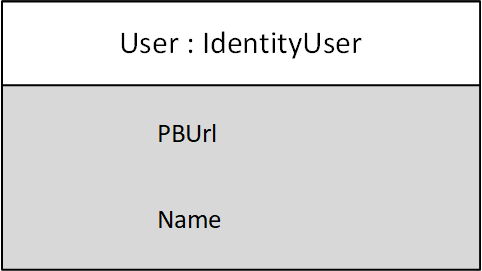
\includegraphics[width=0.45\linewidth]{09_Arkitektur/User/Images/User_DatabaseModel.png}
    \caption{User ER Model}
    \label{fig:ER_Model_User}
\end{figure}

Som der kan ses er der blevet tilføjet et Navn, som er en brugers nickname. Derudover er der sat en string ind til PBUrl. Ud over dette er der blevet lavet 4 relations til entiteterne Groups, WallPosts, GroupsAdministrators samt OwnerGroups.

\mini{Tjek om WallPosts skal fjernes}

\subsection{Logical View}

I logical view for user, er det kun user storien "Indstil profilbillede og personligt tema", som skal implementeres. På baggrund af det meget begrænsede funktionalitet som skal implementeres for user, laves der et kortfattet klassediagram, som kan ses i \ref{fig:UserController_Class}

\begin{figure}[H]
    \centering
    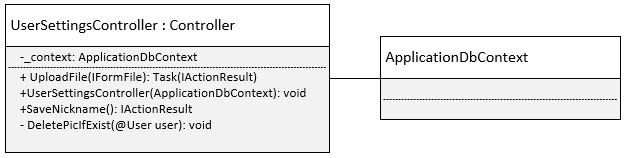
\includegraphics[width=0.9\linewidth]{09_Arkitektur/User/Images/US_Class.JPG}
    \caption{UserController klassediagram: Der ses at klassen har en constructor, som initierer ApplicationDbContexten. Derudover er der en UploadFile action, som er en HttpPost, der modtager en IFormFile, ud fra denne IFormFile kan der udtrækkes profilbilledets data, og skrives ind i projektet, og filstien gemmes i User entiteten.}
    \label{fig:UserController_Class}
\end{figure}

\noindent Temaet er blevet besluttet at blive bygget i \_layout viewet som en drop-down knap, hvor temamulighederne dukket op. Funktionerne som bliver kaldt på disse knapper, bliver skrevet i JavaScript, og fremgår derfor ikke i klassediagrammet.
\section{Gruppe} \label{sec:arch_group}
Arkitekturen for gruppe-funktionaliteter er lavet på baggrund af de US, som er opstillet i afsnit \ref{sec:US}. Det er ikke alle US, som er blevet kigget på, og derfor er det kun følgende funktionaliteter, som der er arbejdet på:
\begin{itemize}
    \item Opret gruppe    
    \item Valg af gruppenavn
    \item Tilføjelse/fjernelse af brugere
    \item Tilføje/fjerne administrator rettigheder
    \item Mulighed for at forlade gruppe
    \item Mulighed for at slette gruppe
    \item Mulighed for at tilføje kælenavnetil medlemmer
    \item Mulighed for at videregive owner rettigheder
\end{itemize}

\noindent Der lægges mest vægt på arkitekturen for US’en "Tilføje/fjerne administrator rettigheder", da denne gennemgås igennem rapporten. \\

\subsection{Data view}
I dette view vises der et ER diagram, som beskriver, hvordan data for grupper og dens medlemmer gemmes i databasen. For en detaljeret beskrivelse af, hvordan der er fundet frem til det følgende ER diagramet på figur \ref{fig:group_ER}, henvises der til bilagene. \thomas{Indset henvisning}.
\thomas{Ret diagram}
\begin{figure}[H]
  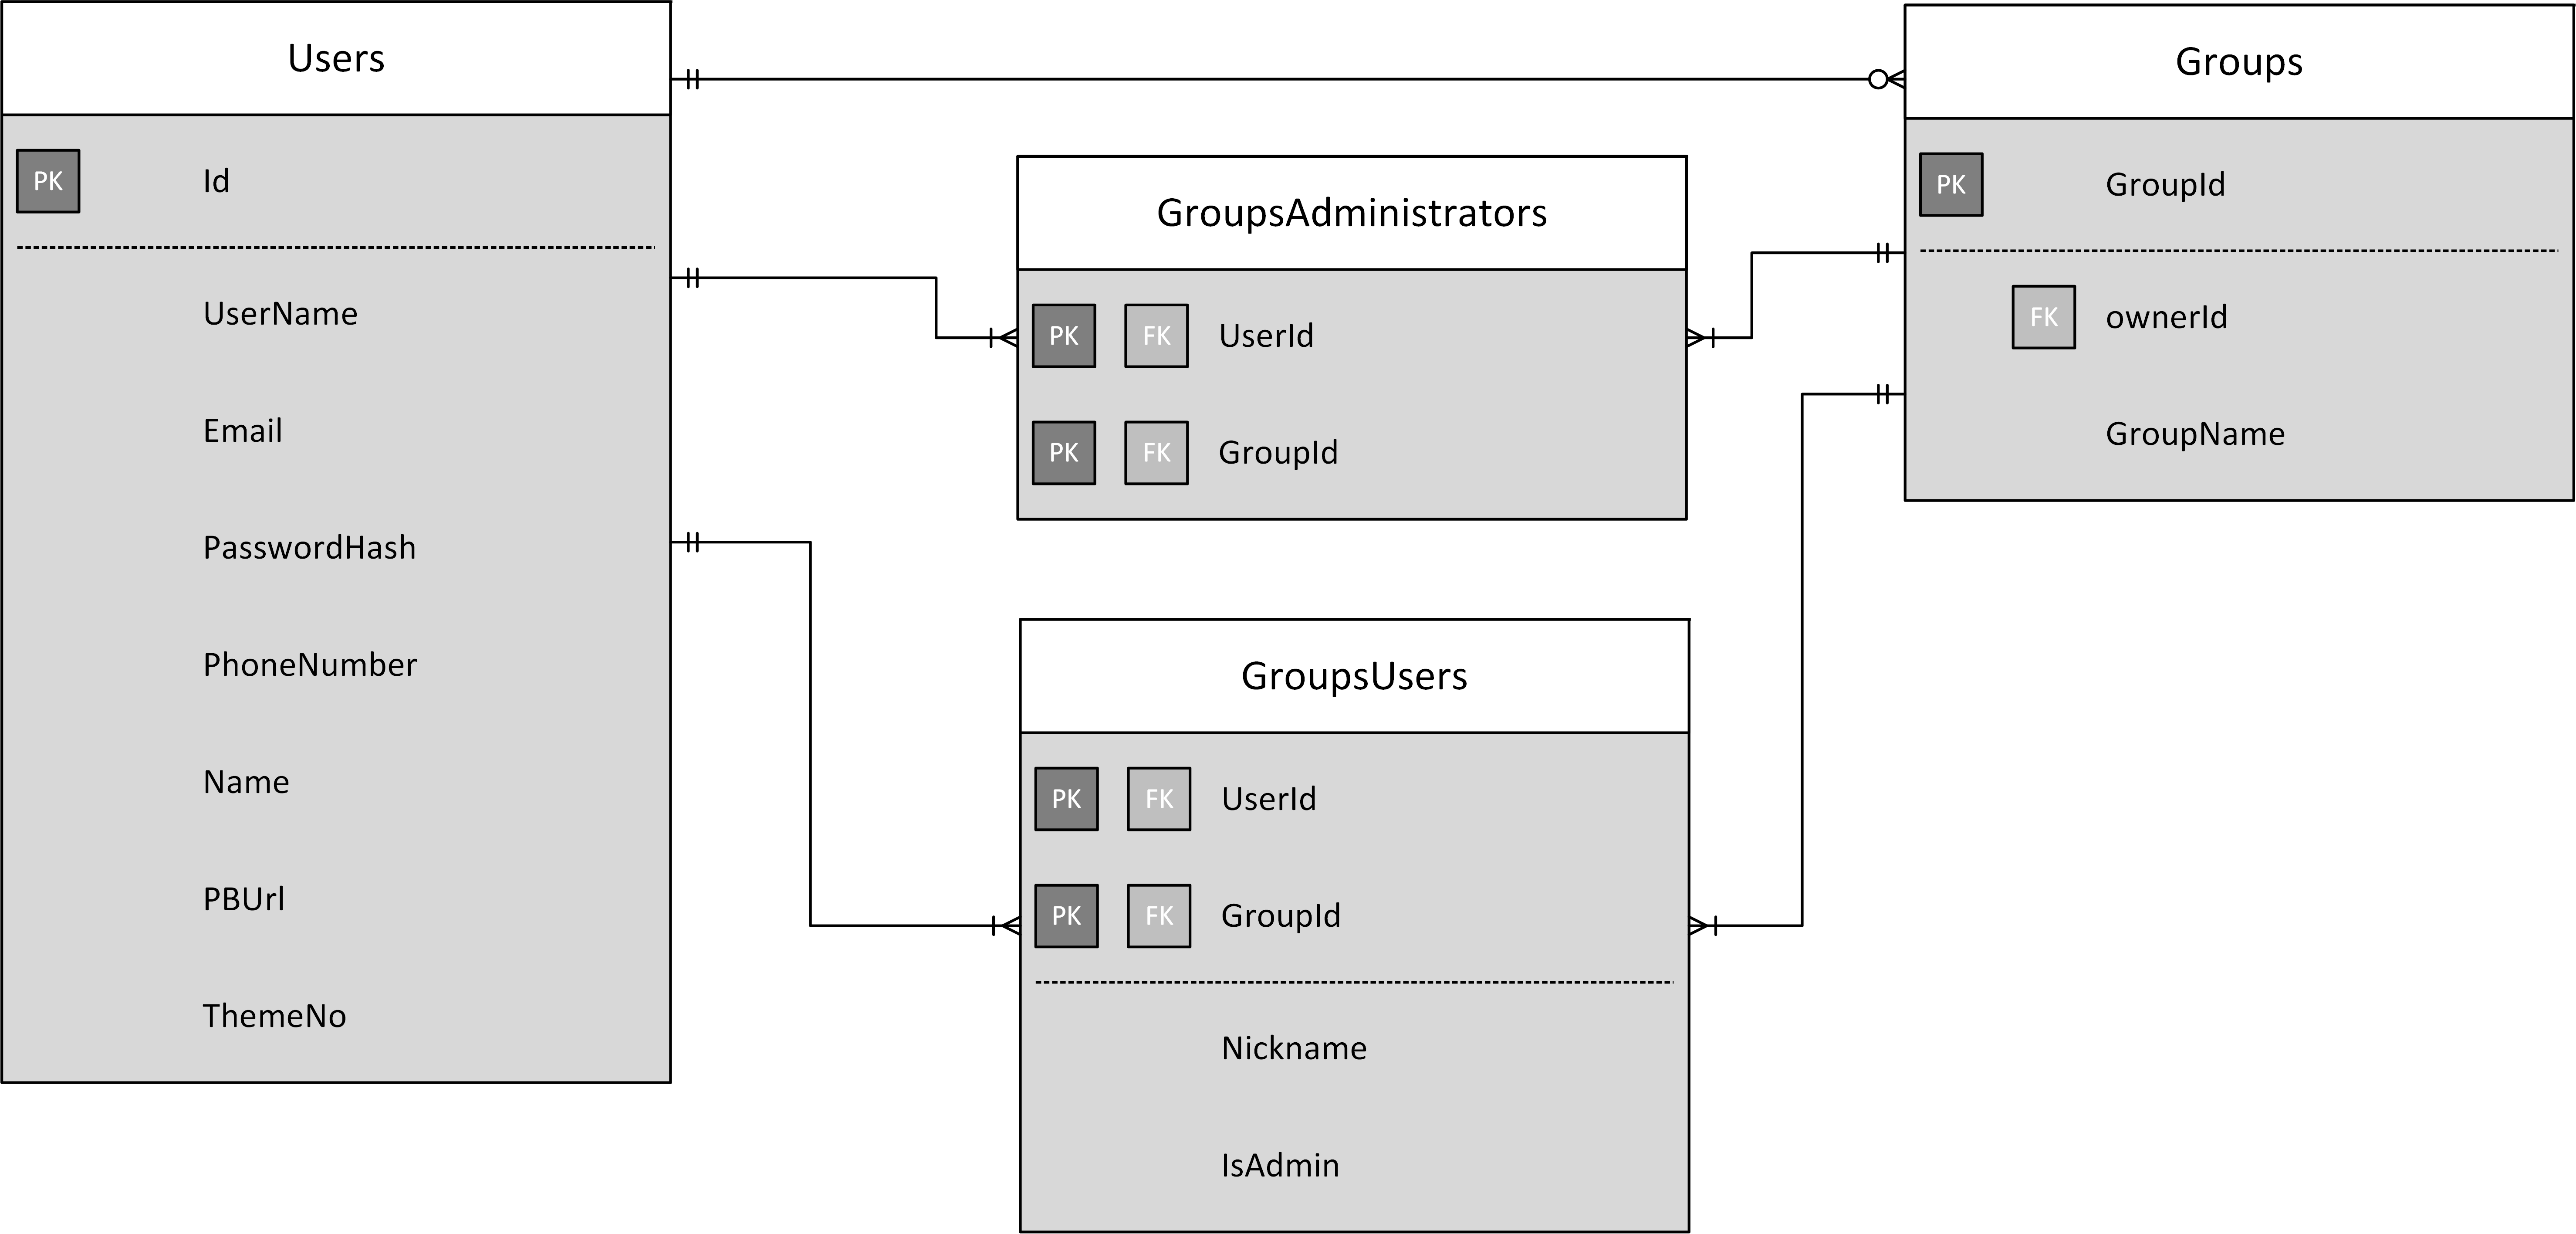
\includegraphics[width=\linewidth]{01_Billeder/09_Arkitektur/Group/Data_Group.png}
  \centering
  \caption{ER Diagram af Groups. Måden det er lavet på, gør at det er muligt at gemme grupper, og deres medlemmer og adminstratorer. Sent i projektet blev det opdaget at tabellen GroupsAdministrators godt kan virke overflødig.}
  \label{fig:group_ER}
\end{figure}

\jonathan{Ændrer rækkefølge på argumenter for GroupAdmins, så det positive ved entiteten kommer først - vidste ikke lige hvordan jeg skulle skrive det.}
\noindent Overflødigheden af GroupAdministrators skyldes at der i GroupsUsers bliver gemt information om hvorvidt et medlem er administrator eller ej. Derfor er der ingen grund til at gemme denne information igen i en anden tabel, da det også bruger plads i databasen. Fordelen ved tabellen er dog at det er hurtigere at finde frem til gruppens administratorer. \\

\subsection{Logical view}
I dette view udarbejdes en controller og views, så US’s til grupper kan blive realiseret. Her bliver det kun vist, hvordan arkitekturen for US’en "Tilføje/fjerne administrator rettigheder" laves, og resten kan findes i bilag. \thomas{indsæt henvisning} \\

\noindent Ideen er, at hjemmesiden skal være nem at bruge, og at der ikke skal navigeres rundt i for mange sider. Derfor er mange af indstillingerne til gruppen skrevet ind i det samme view, herunder US’en "Tilføje/fjerne administrator rettigheder", og der skal være nem adgang til dette view.

\begin{figure}[H]
  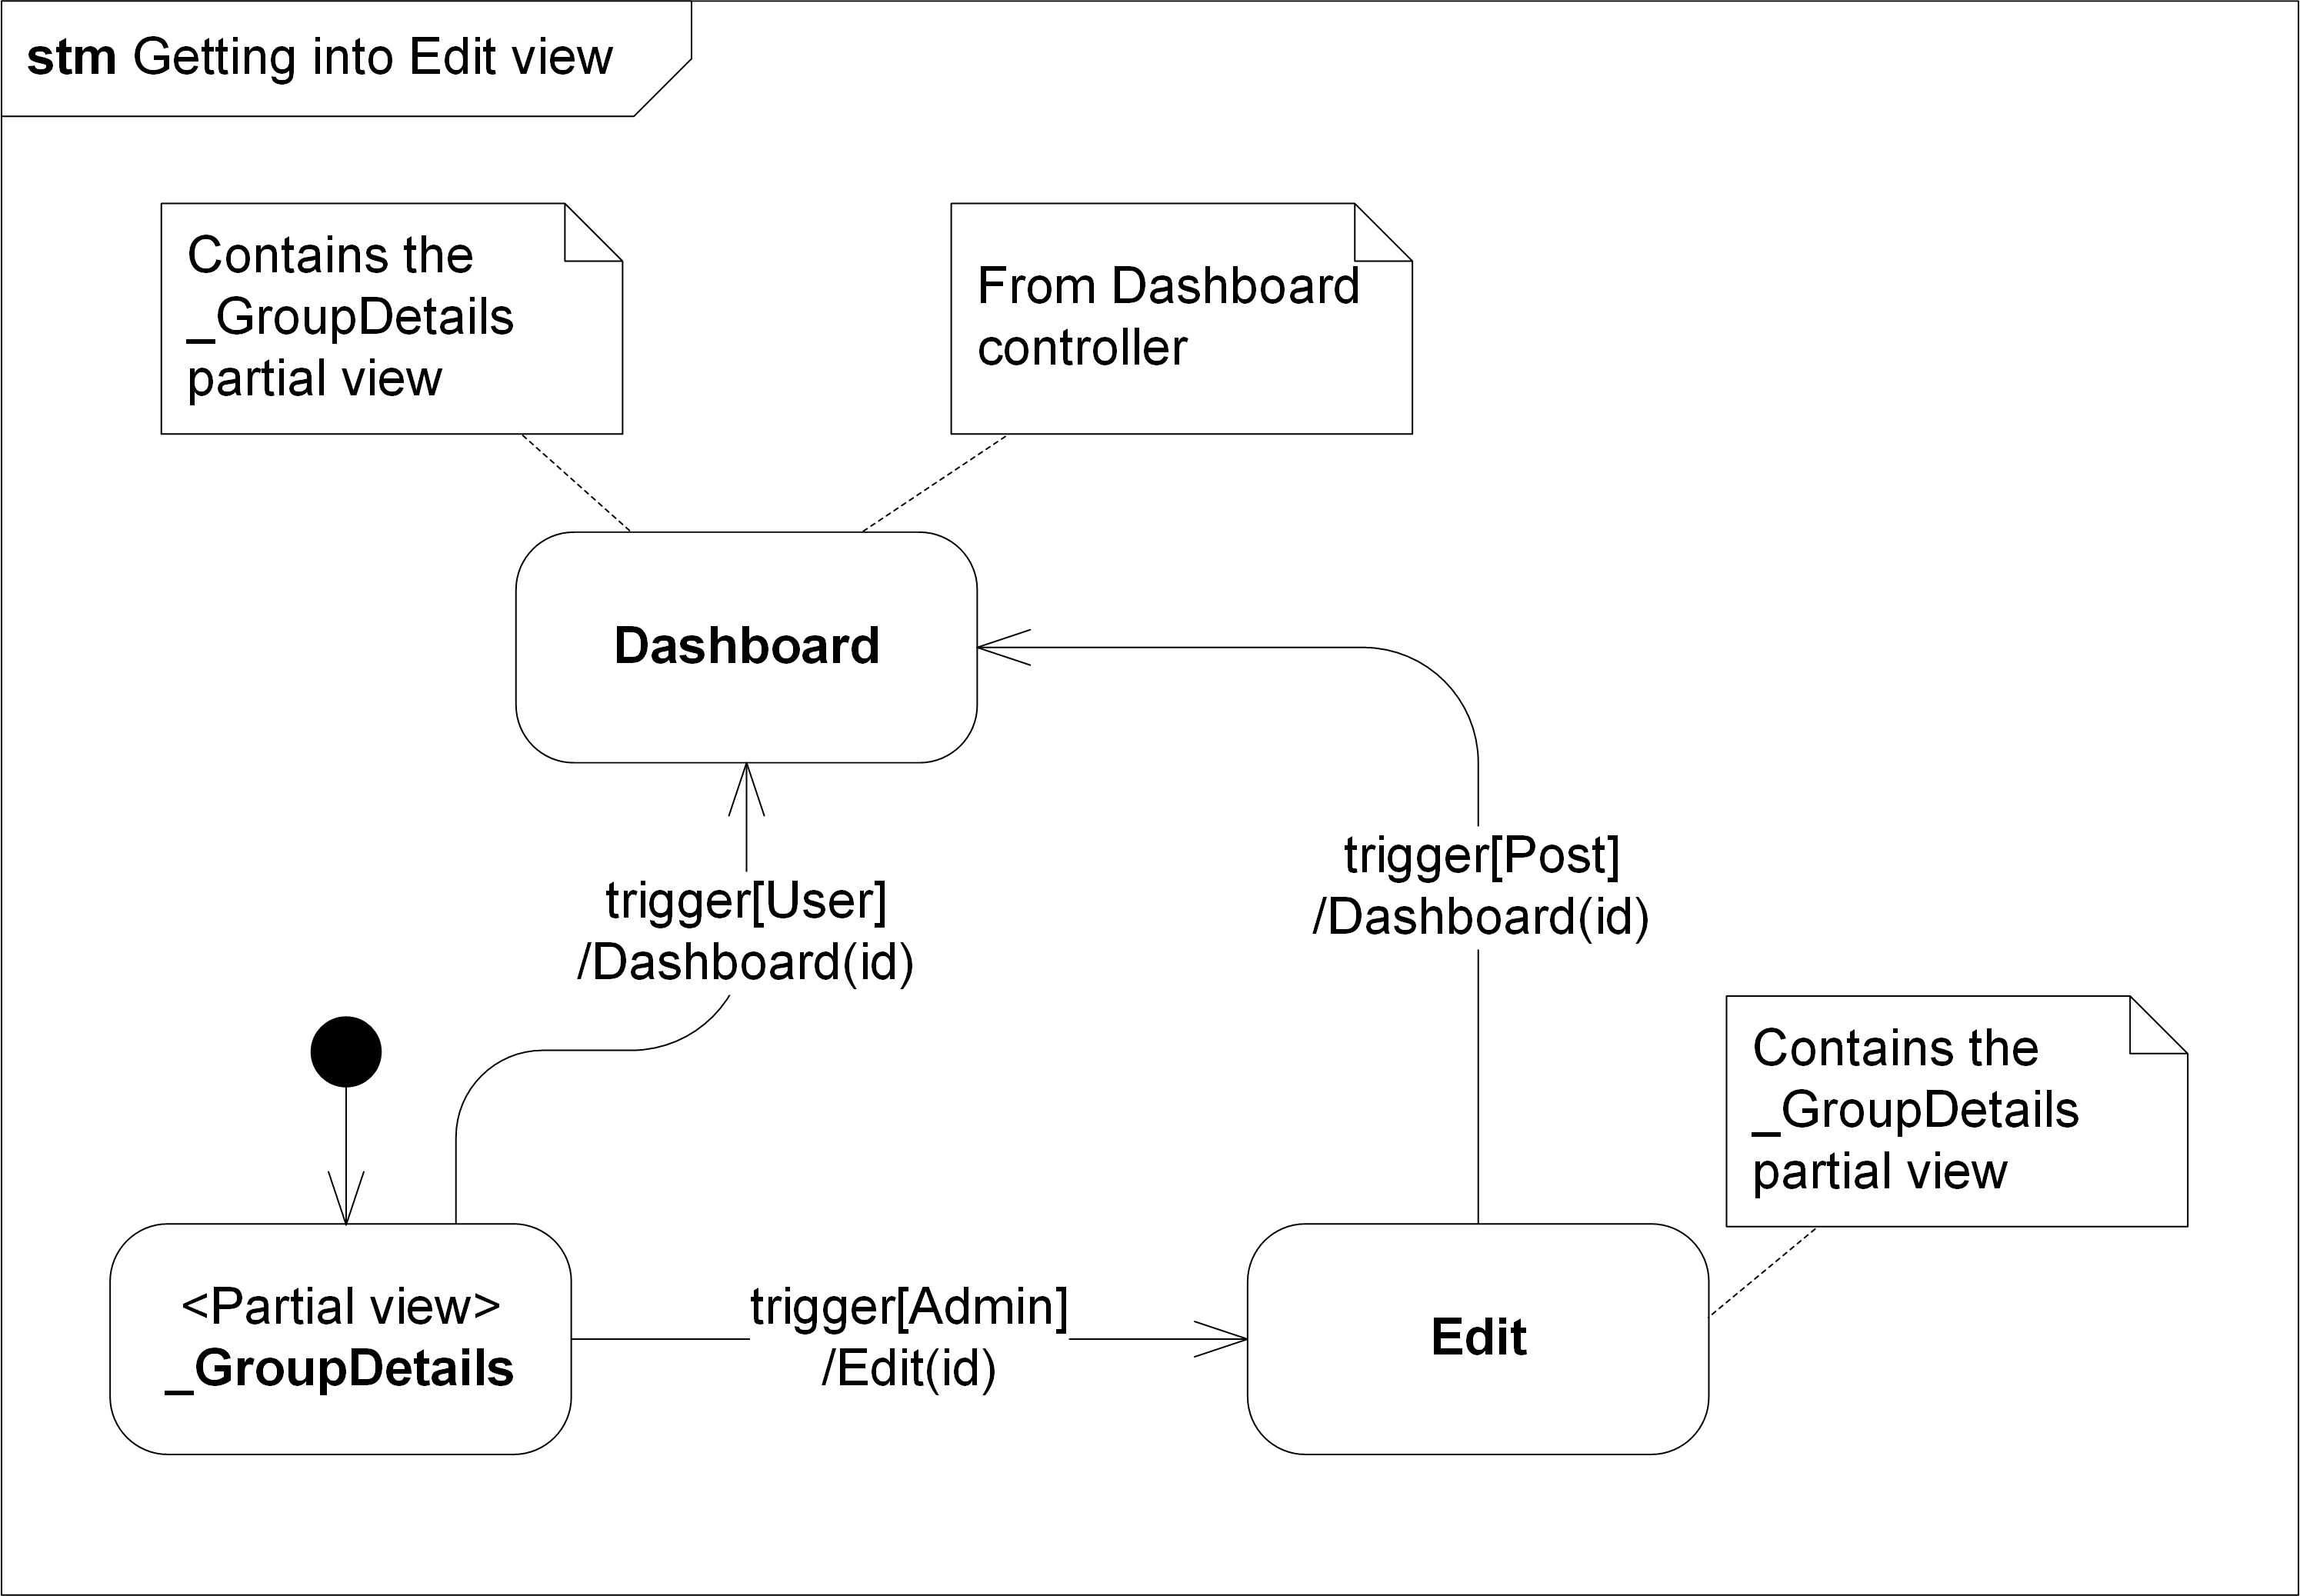
\includegraphics[width=\linewidth]{01_Billeder/09_Arkitektur/Group/LogicalView_Add_Remove_Admin.png}
  \centering
  \caption{Statemachine diagram som viser hvordan man kommer ind i Edit viewet fra \_GroupDetails. Både Edit viewet og Dashboard viewet indeholder \_GroupDetails viewet, og man kan derfor det samme i Edit og Dashboard, som man kan i \_GroupDetails.}
  \label{fig:group_add_remove_admin}
\end{figure}

På figur \ref{fig:group_add_remove_admin} ses Edit viewet, som er viewet, hvor alle gruppens indstillinger kan findes. Herinde skal det være muligt at markere om et medlem er administrator eller ej, ved at markering i en checkboks. Statusen på checkboksen sendes videre til Edit's post funktion, som sørger for at gemme eventuelle ændringer i databasen. På figuren ses der nogle funktionskald mellem de forskellige views. Disse skal skrives ind i klassen GroupController, som kan ses på figur \ref{fig:group_logical_class}.

\begin{figure}[H]
  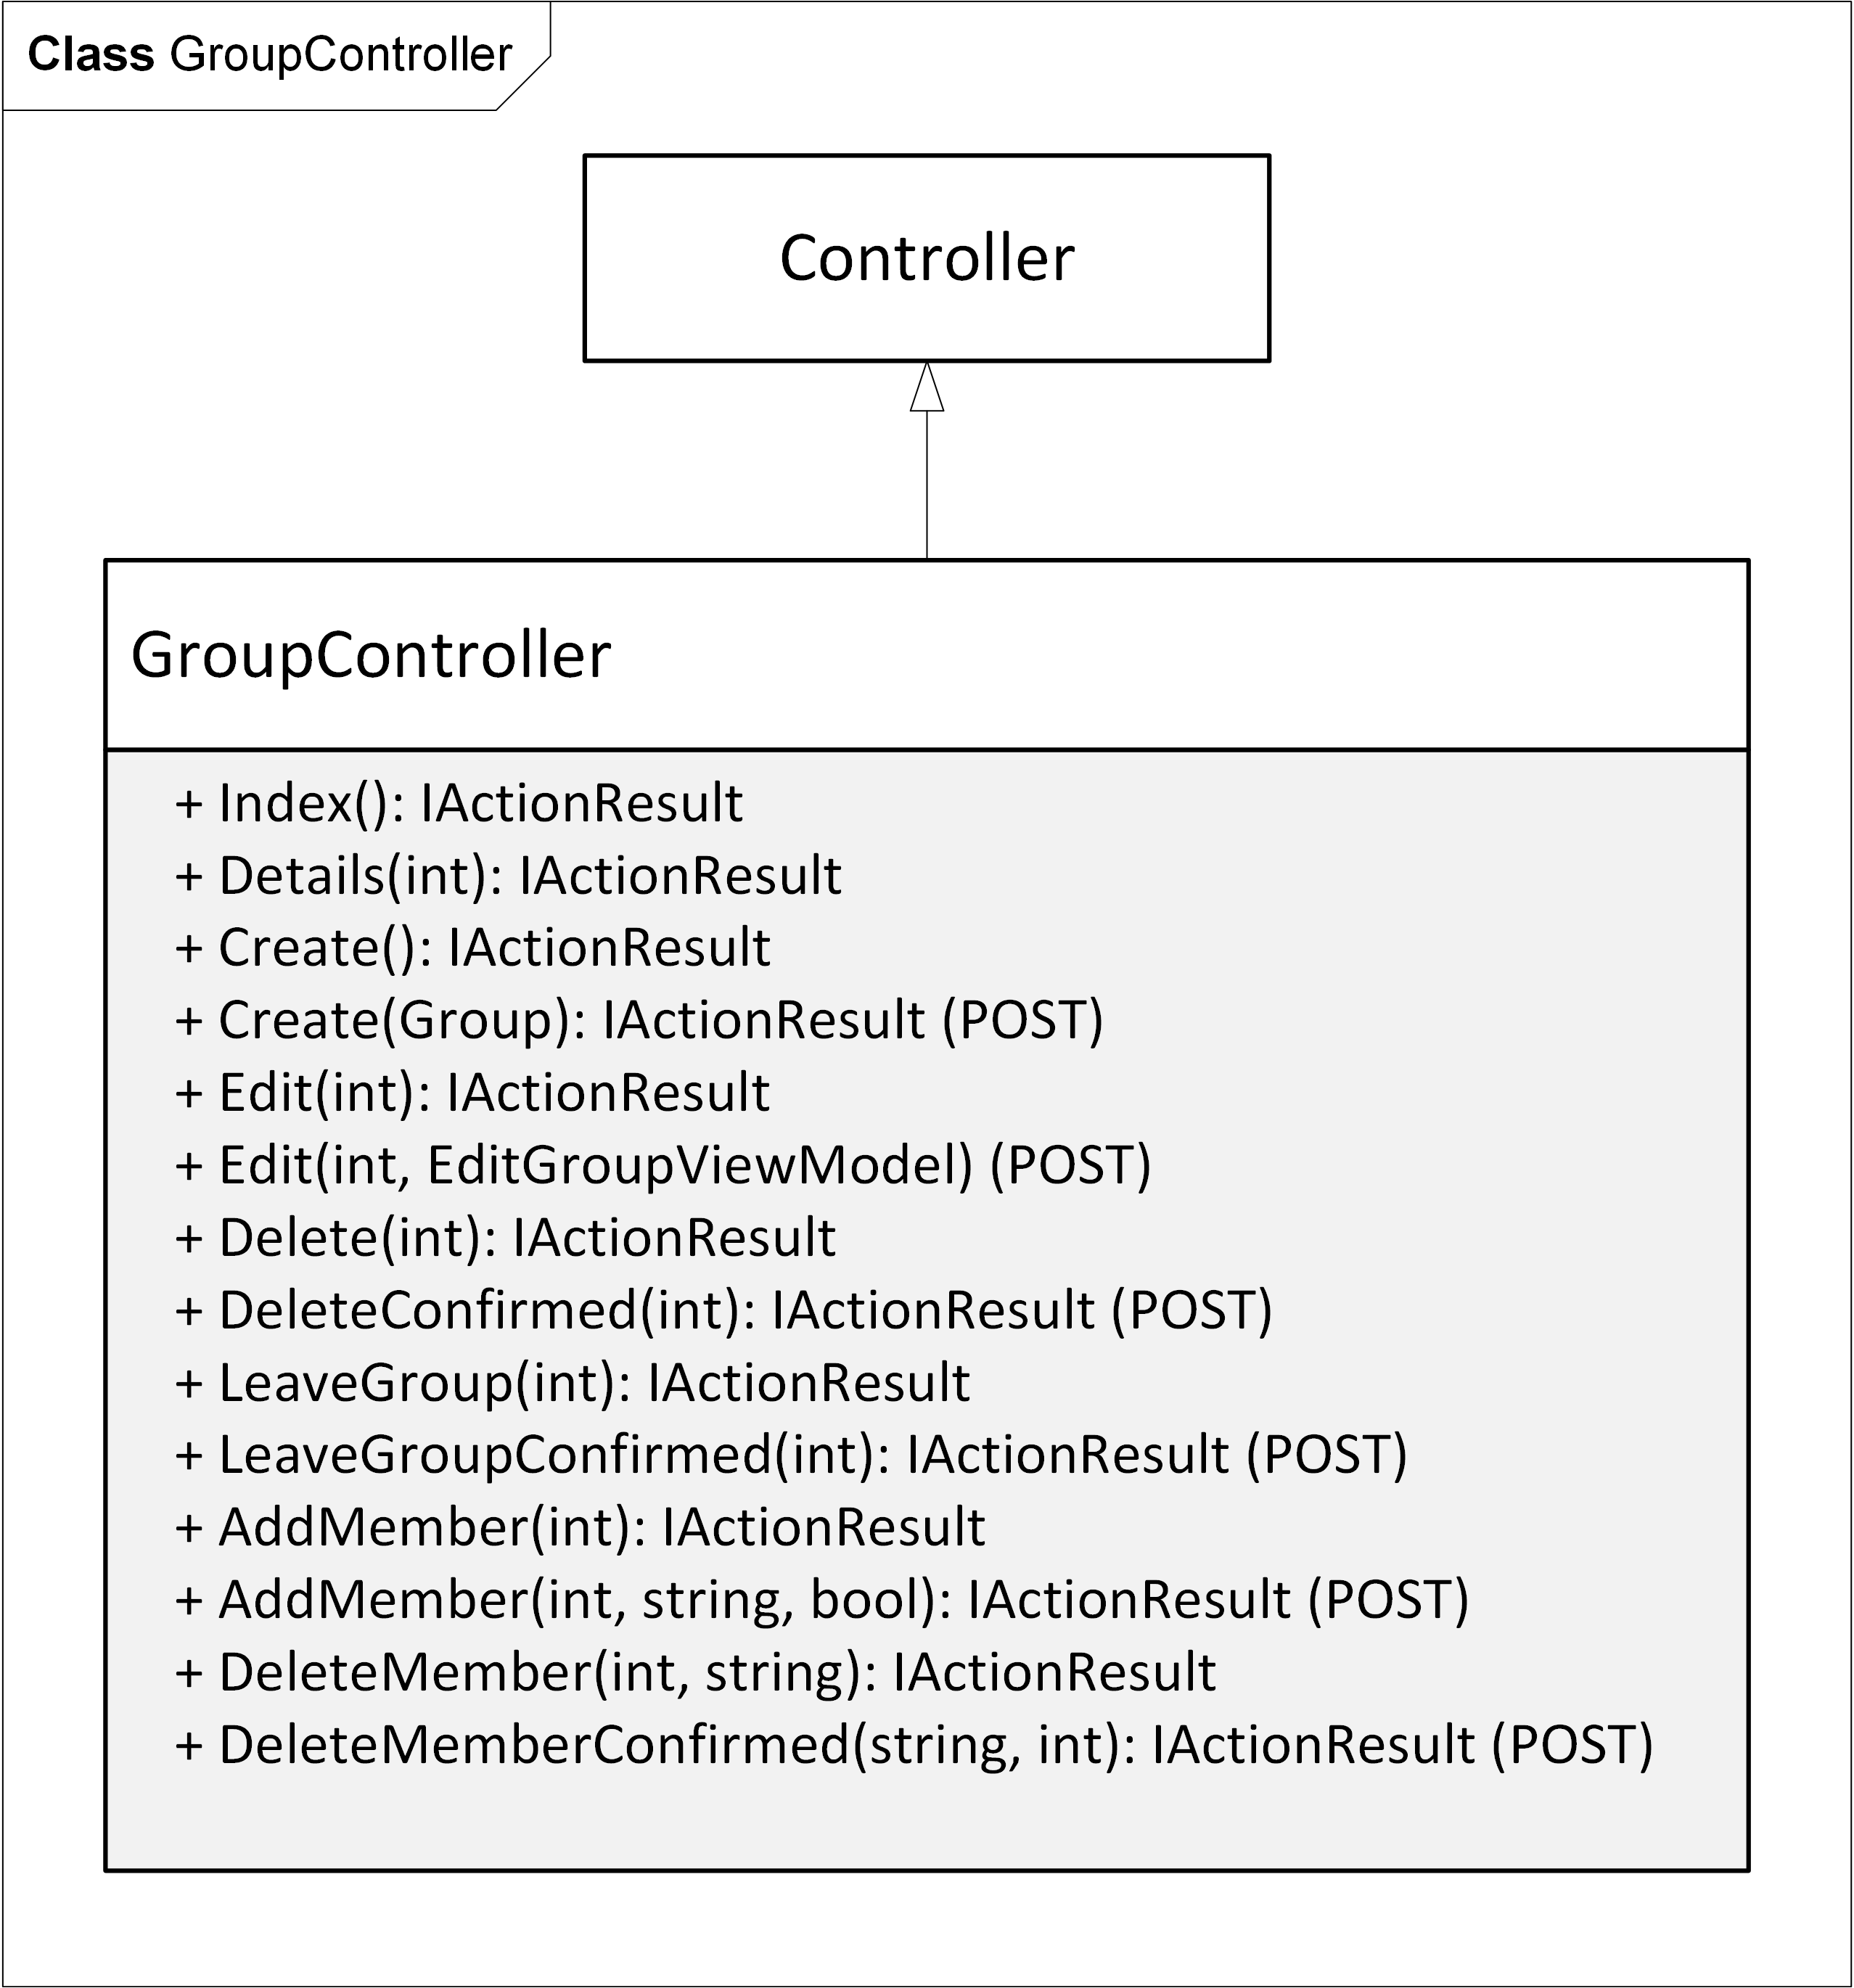
\includegraphics[scale=0.8]{01_Billeder/09_Arkitektur/Group/LogicalView_Class.png}
  \centering
  \caption{Klassediagram af GroupController. Funktioner hvor der står "POST" ud for, er en post funktion for den funktion som står lige over}
  \label{fig:group_logical_class}
\end{figure}

I bilag \thomas{henvisning} ses samme fremgangsmåde brugt på alle US's, som er blevet brugt til at fremstille det samlet klasse diagram for GroupController klassen på figur \ref{fig:group_logical_class}.
\section{Dashboard}
Dashboardet udvikles for at have et sted at samle alle widgets for en gruppe. Det indebærer at linke til de views, hvori man kan redigere og slette de forskellige widgets, herudover skal dashboardet kunne varetage opgaven fra US  tilføj widget, som giver en bruger mulighed for at tilføje/lave en widget til gruppen. US'en "tilføj widget" kan findes på tabel \ref{tab:US_rep}. \\

\begin{figure}[H]
    \centering
    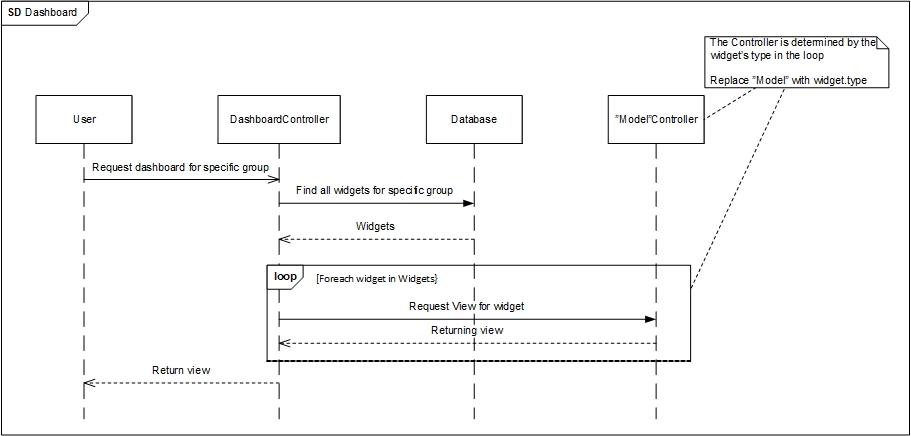
\includegraphics[width=1\textwidth]{09_Arkitektur/Dashboard/Sekvens.jpg}
    \caption{Denne figur viser et sekvensdiagram over udskrivelsen af widgets på dashboard siden. ModelController er herpå figuren udskiftelig med den controller der tilsvare den relevante widget. }
    \label{fig:dashboard_onLoad_seq}
\end{figure}

I det man kommer ind på dashboard siden, loades alle widgets, som set på figur \ref{fig:dashboard_onLoad_seq}. Herefter skal det være muligt at tilføje en widget til gruppens dashboard. Der laves et sekvensdiagram der viser hvordan dette skal foregå, som kan ses på figur \ref{fig:CreateNewWidgetSeq}.

\tobycat{indsæt ref til bilag}
\store{Hvad skal der ref til???}

\begin{figure}[H]
    \centering
    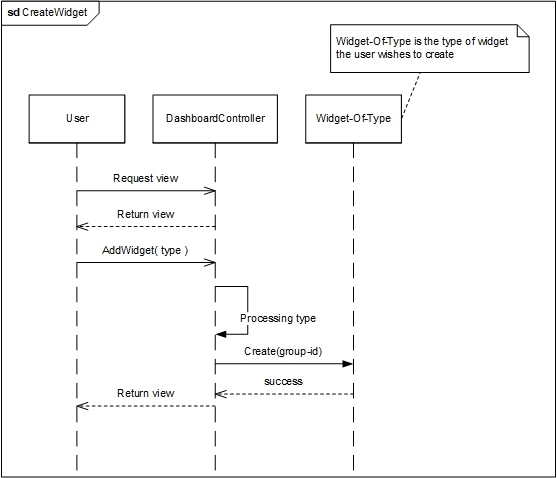
\includegraphics[width=1\textwidth]{09_Arkitektur/Dashboard/CreateWidgetSekvensjpg.jpg}
    \caption{Denne figur viser et sekvensdiagram der beskriver hvordan en vilkårlig widget oprettes. Herpå er widget-of-type lig med den type af widget der skal oprettes}
    \label{fig:CreateNewWidgetSeq}
\end{figure}

\jonathan{der er ikke mellemrum mellem anførselsteg og læses i nedenstående sætning}
Her skal "widget-of-type" læses, som den type af widget, man ønsker at oprette. Dashboardet kalder altså den controller der er tilknyttet den givne type af widget for at oprette en ny widget. Det kan på figuren ses, hvordan DashboardControlleren kommunikere med de andre controllere. Den fulde arkitektur for Dashboard kan findes i bilag \cite{ArkitekturDashboard}.


\section{Booking}
I dette afsnit lægges der mest vægt på arkitekturen for at kunne tilføje/fjerne/redigere ressourcer samt muligheden for at lave automatik gentagende reservationer, da disse gennemgås i rapporten. For at opsummere, skal booking-widgetten kunne følgende:
\begin{itemize}
    \item Tilføje/fjerne/redigere ressourcer
    \item Tilføje/fjerne/redigere reservation af ressource
    \item Mulighed for at lave automatisk gentagende reservationer
    \item Mulighed for at se tilgængelige tider for en ressource i en form for kalender
    \item Mulighed for at synkronisere med kalender
    \item Mulighed for at vælge maksimal antal reservationer pr. periode for en person
\end{itemize}

\subsection{Data view}
Der udarbejdes et ER diagram for de entitier som tilhører Booking systemet. Dette kan ses på figur \ref{fig:Booking_ER}. Dette er den færdige version af ER-diagrammet for Booking-Widgetten. Tidligere versioner for andre iterationer kan findes i bilag. \valdemar{indsæt henvisning og opdater ER diagram}
\begin{figure}[H]
\centering
  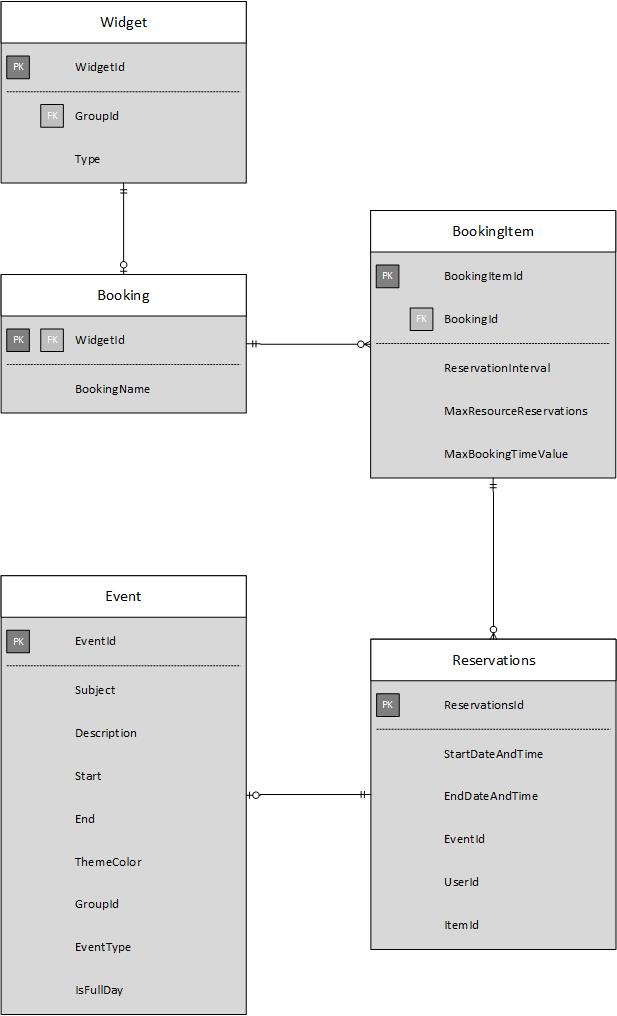
\includegraphics[width=0.5\linewidth]{01_Billeder/09_Arkitektur/Booking.jpg}
  \caption{ER diagram for booking system i databasen. For at kunne tilføje en ressource til et Booking-system, er det nødvendigt at et Booking-system skal have tilknyttet ressourcer(BookingItem). For at der kan foretages reservationer oprettes Reservations, hvor hver reservation tilhører ét BookingItem}
  \label{fig:Booking_ER}
\end{figure}

\subsection{Logical view}
De funktionaliteter der vurderes at blive anvendt oftest, skal være lettest tilgængelige. For at være let tilgængelige bør de kunne anvendes fra widgetten på Dashboardet. Her i rapporten vises der kun diagrammer der er relevante for de to US's som der beskrives i dette afsnit. Resten af diagrammerne kan findes i bilag.

\subsubsection{Tilføj/fjern/redigér ressource}
Arbejdet på de to US's der omhandler at oprette/slette/redigere en ressource, påbegyndes i 4. iteration. Der laves en indledende STM der beskriver hvilke views der kan navigeres rundt i for at oprette/fjerne ressource. Denne kan ses på figur \ref{fig:Booking_STMResource_Initial}
 
\begin{figure}[H]
  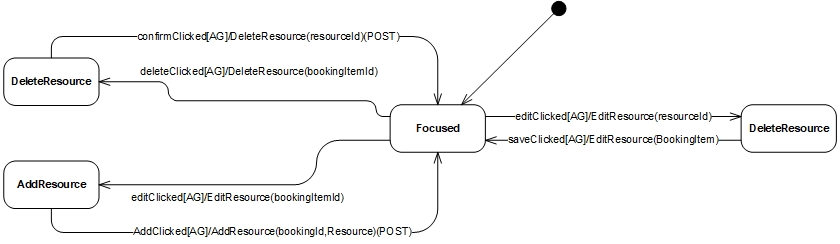
\includegraphics[width=1.0\linewidth]{01_Billeder/09_Arkitektur/STM_AddResource_Initial.jpg}
  \caption{STM fra 4. iteration viser hvordan der kan navigeres mellem forskellige views for at slette/redigere/oprette en ressource. Ordforklaring: AG - Access Granted. For at en bruger kan få adgang til Edit/Delete views, skal brugeren være admin}
  \label{fig:Booking_STMResource_Initial}
\end{figure}

Når widget containeren på dashboardet er klar til kunne anvendes, opdaterers arkitekturen for denne US. Dette gøres i iteration 6. Det vurderes at AddResource Viewet vil blive brugt oftere end Delete/Edit hvormed denne kan tilgås både fra \_Booking viewet og Focused viewet, hvor de to andre views kun kan tilgås fra Focused viewet. Desuden implementeres disse tre views nu som Pop-up vinduer. En STM der viser hvilke views den skal indeholde, og hvordan der kan navigeres mellem disse kan ses på figur \ref{fig:Booking_STMResource_Final}.  

\begin{figure}[H]
  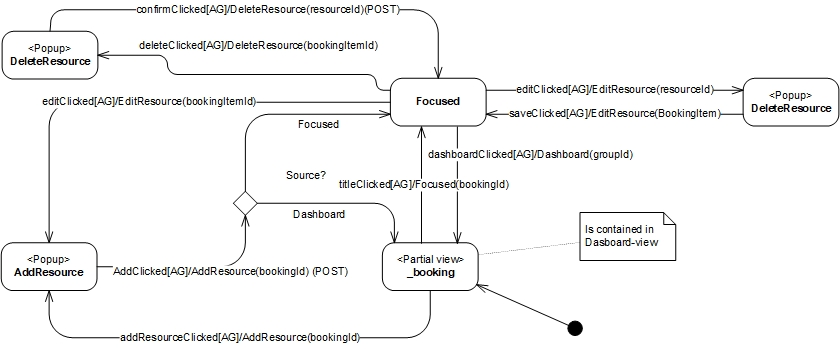
\includegraphics[width=1.0\linewidth]{01_Billeder/09_Arkitektur/STM_AddResource_Final.jpg}
  \caption{STM fra 6. iteration der viser hvordan der kan navigeres mellem forskellige views for at slette/redigere/oprette en ressource. Når POST funktionen kaldes efter der trykkes på 'Confirm', omdirigeres der til det view som pilen peger på. Ordforklaring: AG - Access Granted. For at en bruger kan få adgang til Edit/Delete views, skal brugeren være admin}
  \label{fig:Booking_STMResource_Final}
\end{figure}

\subsubsection{Opret gentagende reservation}
Arkitekturen af denne funktionalitet påbegyndes i iteration 5, efter det er blevet muligt at foretage en enkelt reservation af en ressource. For at kunne oprette en gentagende reservation er det blevet besluttet at skulle være en valgmulighed når der oprettes en enkelt reservation. En STM, fra iteration 5, der beskriver de mulige views som associeres med at oprette en gentagende reservation, kan ses på figur  \ref{fig:Booking_STMReservation_Initial}.   

\begin{figure}[H]
  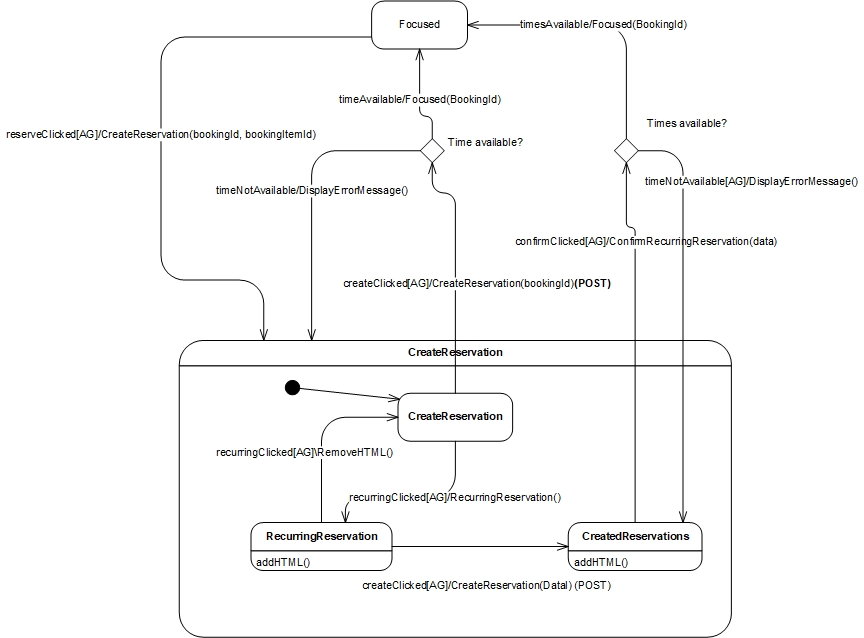
\includegraphics[width=1.0\linewidth]{01_Billeder/09_Arkitektur/STM_CreateReservation_Initial.jpg}
  \caption{STM der viser hvilke views der gør det muligt at oprette en gentagende reservation fra iteration 5. I CreateReservaition viewet repræsenterer der forskellige states, hvilket indold der vises. addHTML og removeHTML funktionerne viser hvornår der tilføjes/fjernes indhold. Ordforklaring: AG - AccessGranted}
  \label{fig:Booking_STMReservation_Initial}
\end{figure}
 Hvis der vælges at der skal foretages gentagende reservationer, hentes indhold fra serveren som indeholder valgmuligheder for at foretage gentagende reservationer. Efter brugeren trykker på create-knappen sendes information tilbage til serveren omkring brugerens ønskede reservationer. Serveren finder da ud af hvilke reservationer er mulige, og sender da denne information tilbage til klienten, som da vises på skærmen. Brugeren skal da bekræfte reservationerne. Afhængig af om tiderne stadig er ledige, omdirigeres til Focused viewet, eller der vises en fejlbesked.
Alle disse skridt er nødvendige for at sikre at der ikke kan foretages reservationer, hvor en ressource er reserveret af en anden bruger.

I 6. iteration, når widgetten containeren bliver klar, opdateres arkitekturen for denne US. Her laves siden hvor der foretages gentagende reservationer, om til et pop-up vindue. Desuden bliver det muligt at tilgå denne funktionalitet fra en Booking-widget fra dashboard. En STM der viser dette kan ses på figur \ref{fig:Booking_STMReservation_Final}. Den præcis samme funktionalitet er tilgængelig fra Focused viewet, men vises ikke her, da dette ville være overflødigt. 

\begin{figure}[H]
  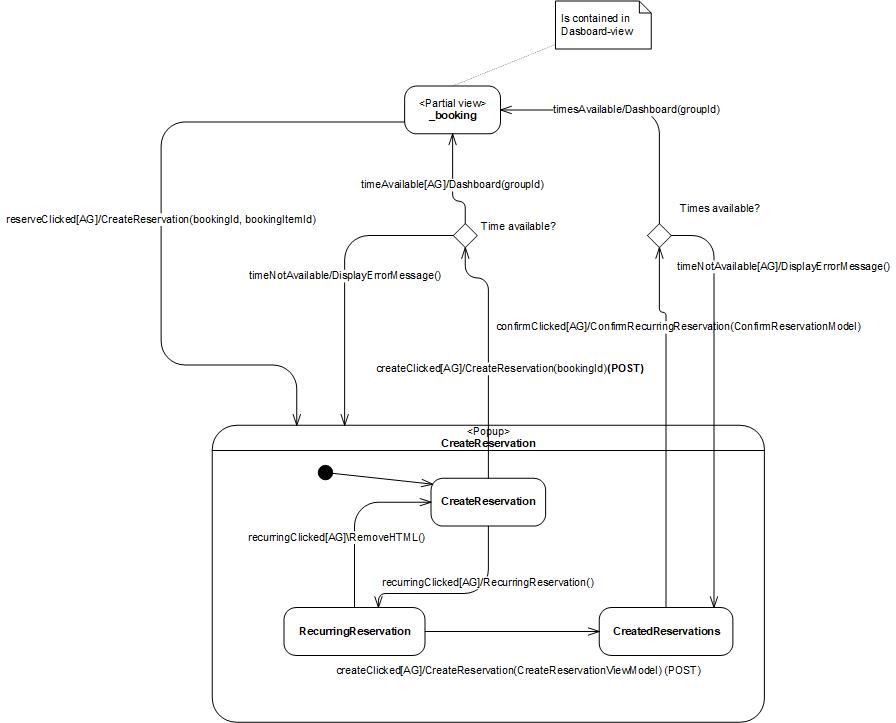
\includegraphics[width=1.0\linewidth]{01_Billeder/09_Arkitektur/STM_CreateReservationReport.jpg}
  \caption{STM der viser hvilke views der gør det muligt at oprette en gentagende reservation fra en Booking-widget i dashboardet for iteration 6. Når brugeren opretter de gentagende reservationer, omdirigeres atomatisk til den side som reservationerne blev foretaget fra.  Ordforklaring: AG - AccessGranted}
  \label{fig:Booking_STMReservation_Final}
\end{figure}

Restriktionen om at allerede reserveret ressource ikke skal kunne reserveres, går igen i hele arkitekturen for Booking. STM's for den resterende arkitektur kan findes i bilag. 
\valdemar{Skal indsætte reference til bilag}











\section{Calendar}

Eftersom calendar skal have mulighed for at have personlig, samt fælles visning for en hel gruppe som widget, blev der besluttet at den personlige skulle være nem at navigere til, og er derfor blevet placeret i hjemmesidens navbar. Af denne grund er det blevet besluttet at lave to controllere, en GroupCalendar samt en Calendar til personlig visning. For at opsummere hvad kalenderens funktionalitet skal indebære, kan der herunder ses de user stories som calendar er en del af:

\begin{itemize}
    \item Tilføj/fjern begivenheder
    \item Valg af filter
    \item Skift mode (fælles/personlig)
    \item Valg af visning
    \item Mulighed for synkronisering med Google Calendar *
\end{itemize}

*Ikke implementeret

På nedenstående tabel ses, hvilken funktionalitet der er for begge kalendere.

%GroupCalendar laves som widget, og har derfor CRUD funktioner som den personlige ikke har, og den personlige har heller ikke mulighed for at indsætte events, da events skal tilknyttes en gruppe. \newline


\noindent  
\begin{tabular}{|p{2.0in}|p{1.5in}|p{1.5in}|} \hline 
\textbf{} & \textbf{Gruppe kalender} & \textbf{Personlig kalender}\\ \hline 
Overblik af en gruppes events & x & x \\ \hline
Overblik over events for alle grupper, bruger er medlem af &  & x \\ \hline 
Widget & x &  \\ \hline 
Tilf{\o}je begivenheder & x &  \\ \hline 
Slette begivenheder & x & \\ \hline 
Valg af visning & x & x \\ \hline
CRUD funktioner for widget & x &  \\ \hline
\end{tabular}
\noindent 



\subsection{Data view}

I første iteration af arbejdet med kalenderen blev der kun gemt events i databasen, eftersom det er det eneste som behøves i databasen for at få kalenderen til at virke. Alle events har gruppeID, og de kan på denne måde findes til hver gruppe på denne måde. Hvis systemet bliver populært, kan dette dog hurtigt blive et problem, at skulle iterere igennem alle events i hele databasen. I senere iterationer skulle kalenderen laves til widget, og der blev i denne forbindelse gemt en liste af events for hver calendar widget, hvori man så blot finder events ud fra denne liste. I bilag \cite{ArkitekturCalendar} kan der læses mere om dette, hvori der også kan ses data access layer.

\begin{figure}[H]
    \centering
    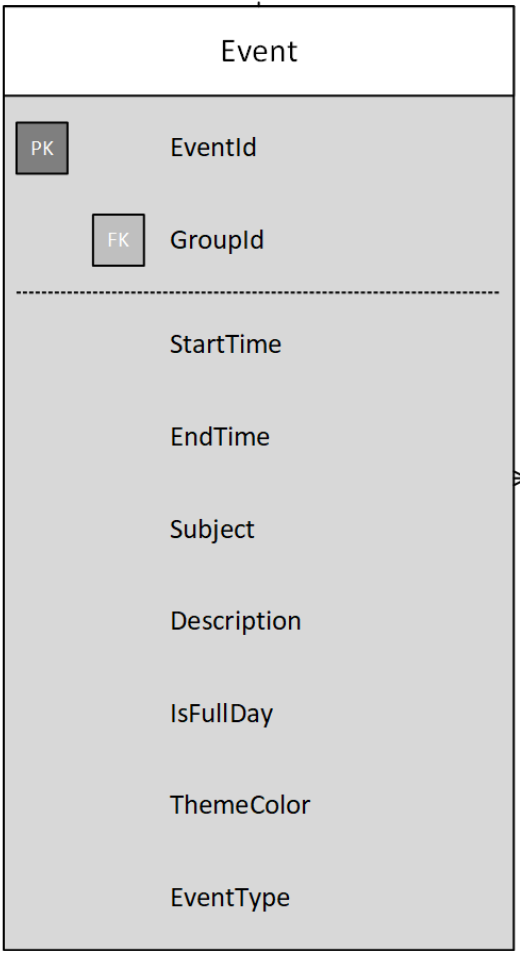
\includegraphics[width=0.25\linewidth]{09_Arkitektur/Calendar/Images/EventData.png}
    \caption{Event database model. Det kan ses GroupId er en foreign key, hvilket kan bruges til at finde de events der findes for en bestemt gruppe}
    \label{fig:eventDB}
\end{figure}

\subsection{Logical view}

Da der blev undersøgt hvordan der kunne laves en kalender, blev der fundet siden "fullcalendar.io", som er en populær javascript baseret kalender med fine stylesheets, og som gratis kan benyttes \cite{Fullcalendar}. fullcalendar.io har desuden valg af dag/uge/måned visning indbygget, hvilket er en user story for kalenderen. Hertil er der lavet et javascript "GroupCalendar.js", som henter events ned i kalenderen fra URL'en /GroupCalendar/GetEvents/(int id, string type), som er en action der returnerer et JSON result. Ud fra disse events, noteret på JSON format, så dannes kalenderen. 
For at overholde kravene noteret i user stories, er der derudover kommet frem til klassediagrammet i figur \ref{fig:CalendarControllerClass}.

\begin{figure}[H]
    \centering
    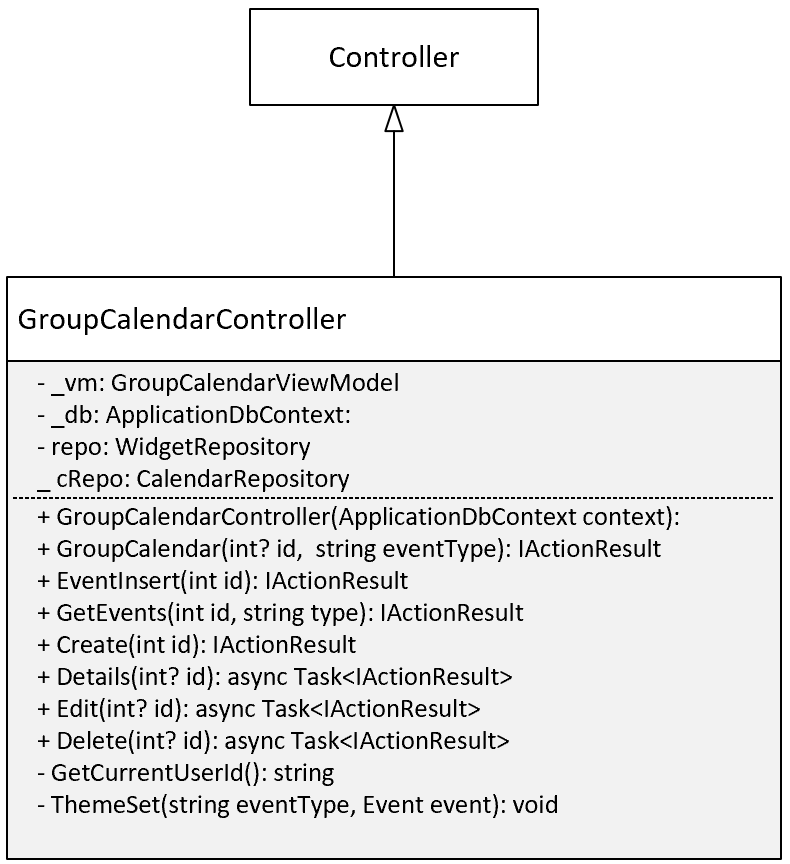
\includegraphics[width=0.5\linewidth]{09_Arkitektur/Calendar/Images/CalendarController.png}
    \caption{Figuren viser CalendarController klassediagrammet. Det ses at der er en GroupCalendarViewModel, som indeholder information til at danne URL'en som "GroupCalendar.js" henter events fra. Til Data Access Layer benyttes Widget og CalendarRepository }
    \label{fig:CalendarControllerClass}
\end{figure}{}

Hovedsageligt benyttes repository til DAL, bla. for at overholde SRP, men til små mindre kald til databasen, som ikke giver mening at lave en metode til i repository, benyttes ApplicationDbContext. \newline
\section{List}

I dette afsnit vil arkitekturen for widgettypen List blive præsenteret. Dette vil ligge grundlag for at en uddybende beskrivelse af hvordan widget'en er designet og implementeret.

List har været under udvikling næsten hele semestret, hvor sidste prik over i'et blev sat under 6. iteration. Udviklingen af List kan afspejles i nedenstående figur, der viser hvilket funktionaliteter List har fået under forskellige iterationer.

\begin{figure}[H]
    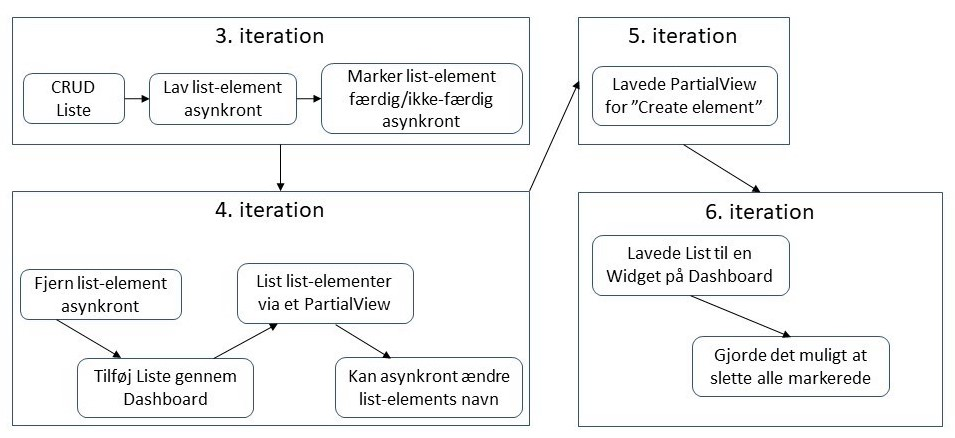
\includegraphics[width=\linewidth]{09_Arkitektur/Lists/Images/Iterationer.jpg}
    \caption{Figuren viser hvordan List har været under udvikling i lang til. Dette afspejler meget at udviklingen har givet mere viden undervejs, hvilket har ledt til optimering.}
    \label{fig:ListIterationer}
\end{figure}

I den sidste iteration blev der også gjort sådan at ListItems bliver streget ud gennem JavaScript inden der modtages et nyt PartialView fra serveren.

\subsection{Data view}

Relationen mellem en liste og dens list-elementer er en-til-mange, da en liste skal kunne have mange ListItems. En ListItem har en composite key, som består af ListId og ListItemId, hvilket giver en god dataintegritet, sådan at de ListItems der bliver vist rent faktisk tilhører den samme liste.

\begin{figure}[H]
    \centering
    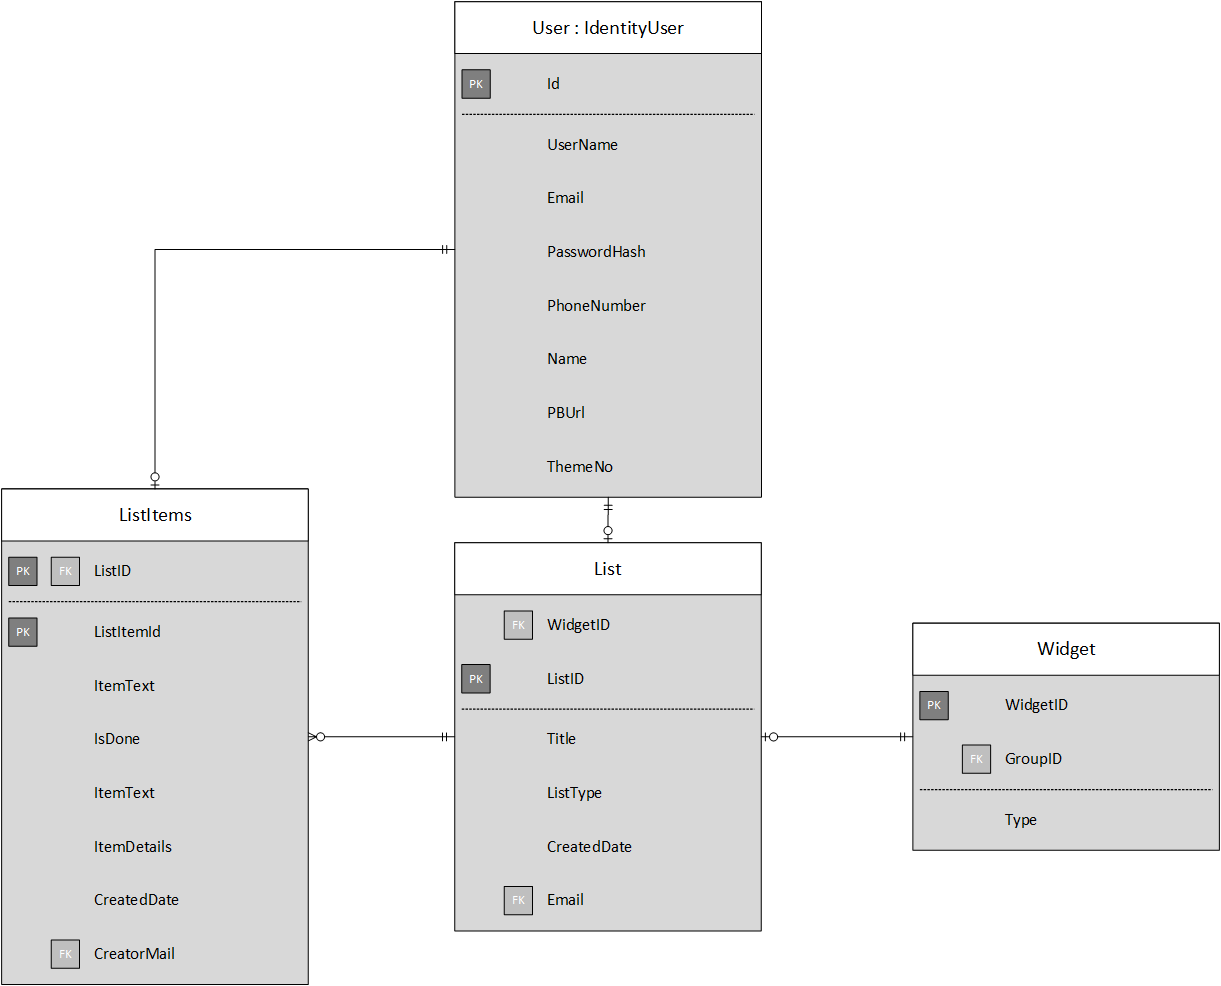
\includegraphics[width=0.9\linewidth]{09_Arkitektur/Lists/Images/ListDbFinal.png}
    \caption{Da List har været under udvikling i mange iterationer, har dataen for List også ændret sig. Bl.a. ListType og CreatorMail er noget der er blevet tilføjet løbende.}
    \label{fig:ListDbFinal}
\end{figure}

CreatorMail for en ListItem er specielt hensigtsmæssig, så man kan se hvem der har lavet list elementet. 

\subsection{Logical view}

List har forholdsvis mange funktionaliteter gemt i sig. En widget har ikke meget plads på dashboard, og det er derfor begrænset hvad der kan være i den lille boks. Selvom det er gjort muligt at udvide boksende, er det dog stadig at foretrække at alt kan ses direkte, i stedet for at skulle folde den ud. På nedestående figur ses arkitektur for hvordan alle funktionaliteterne er wrappet sammen ud fra én fokuseret liste.

\begin{figure}[H]
    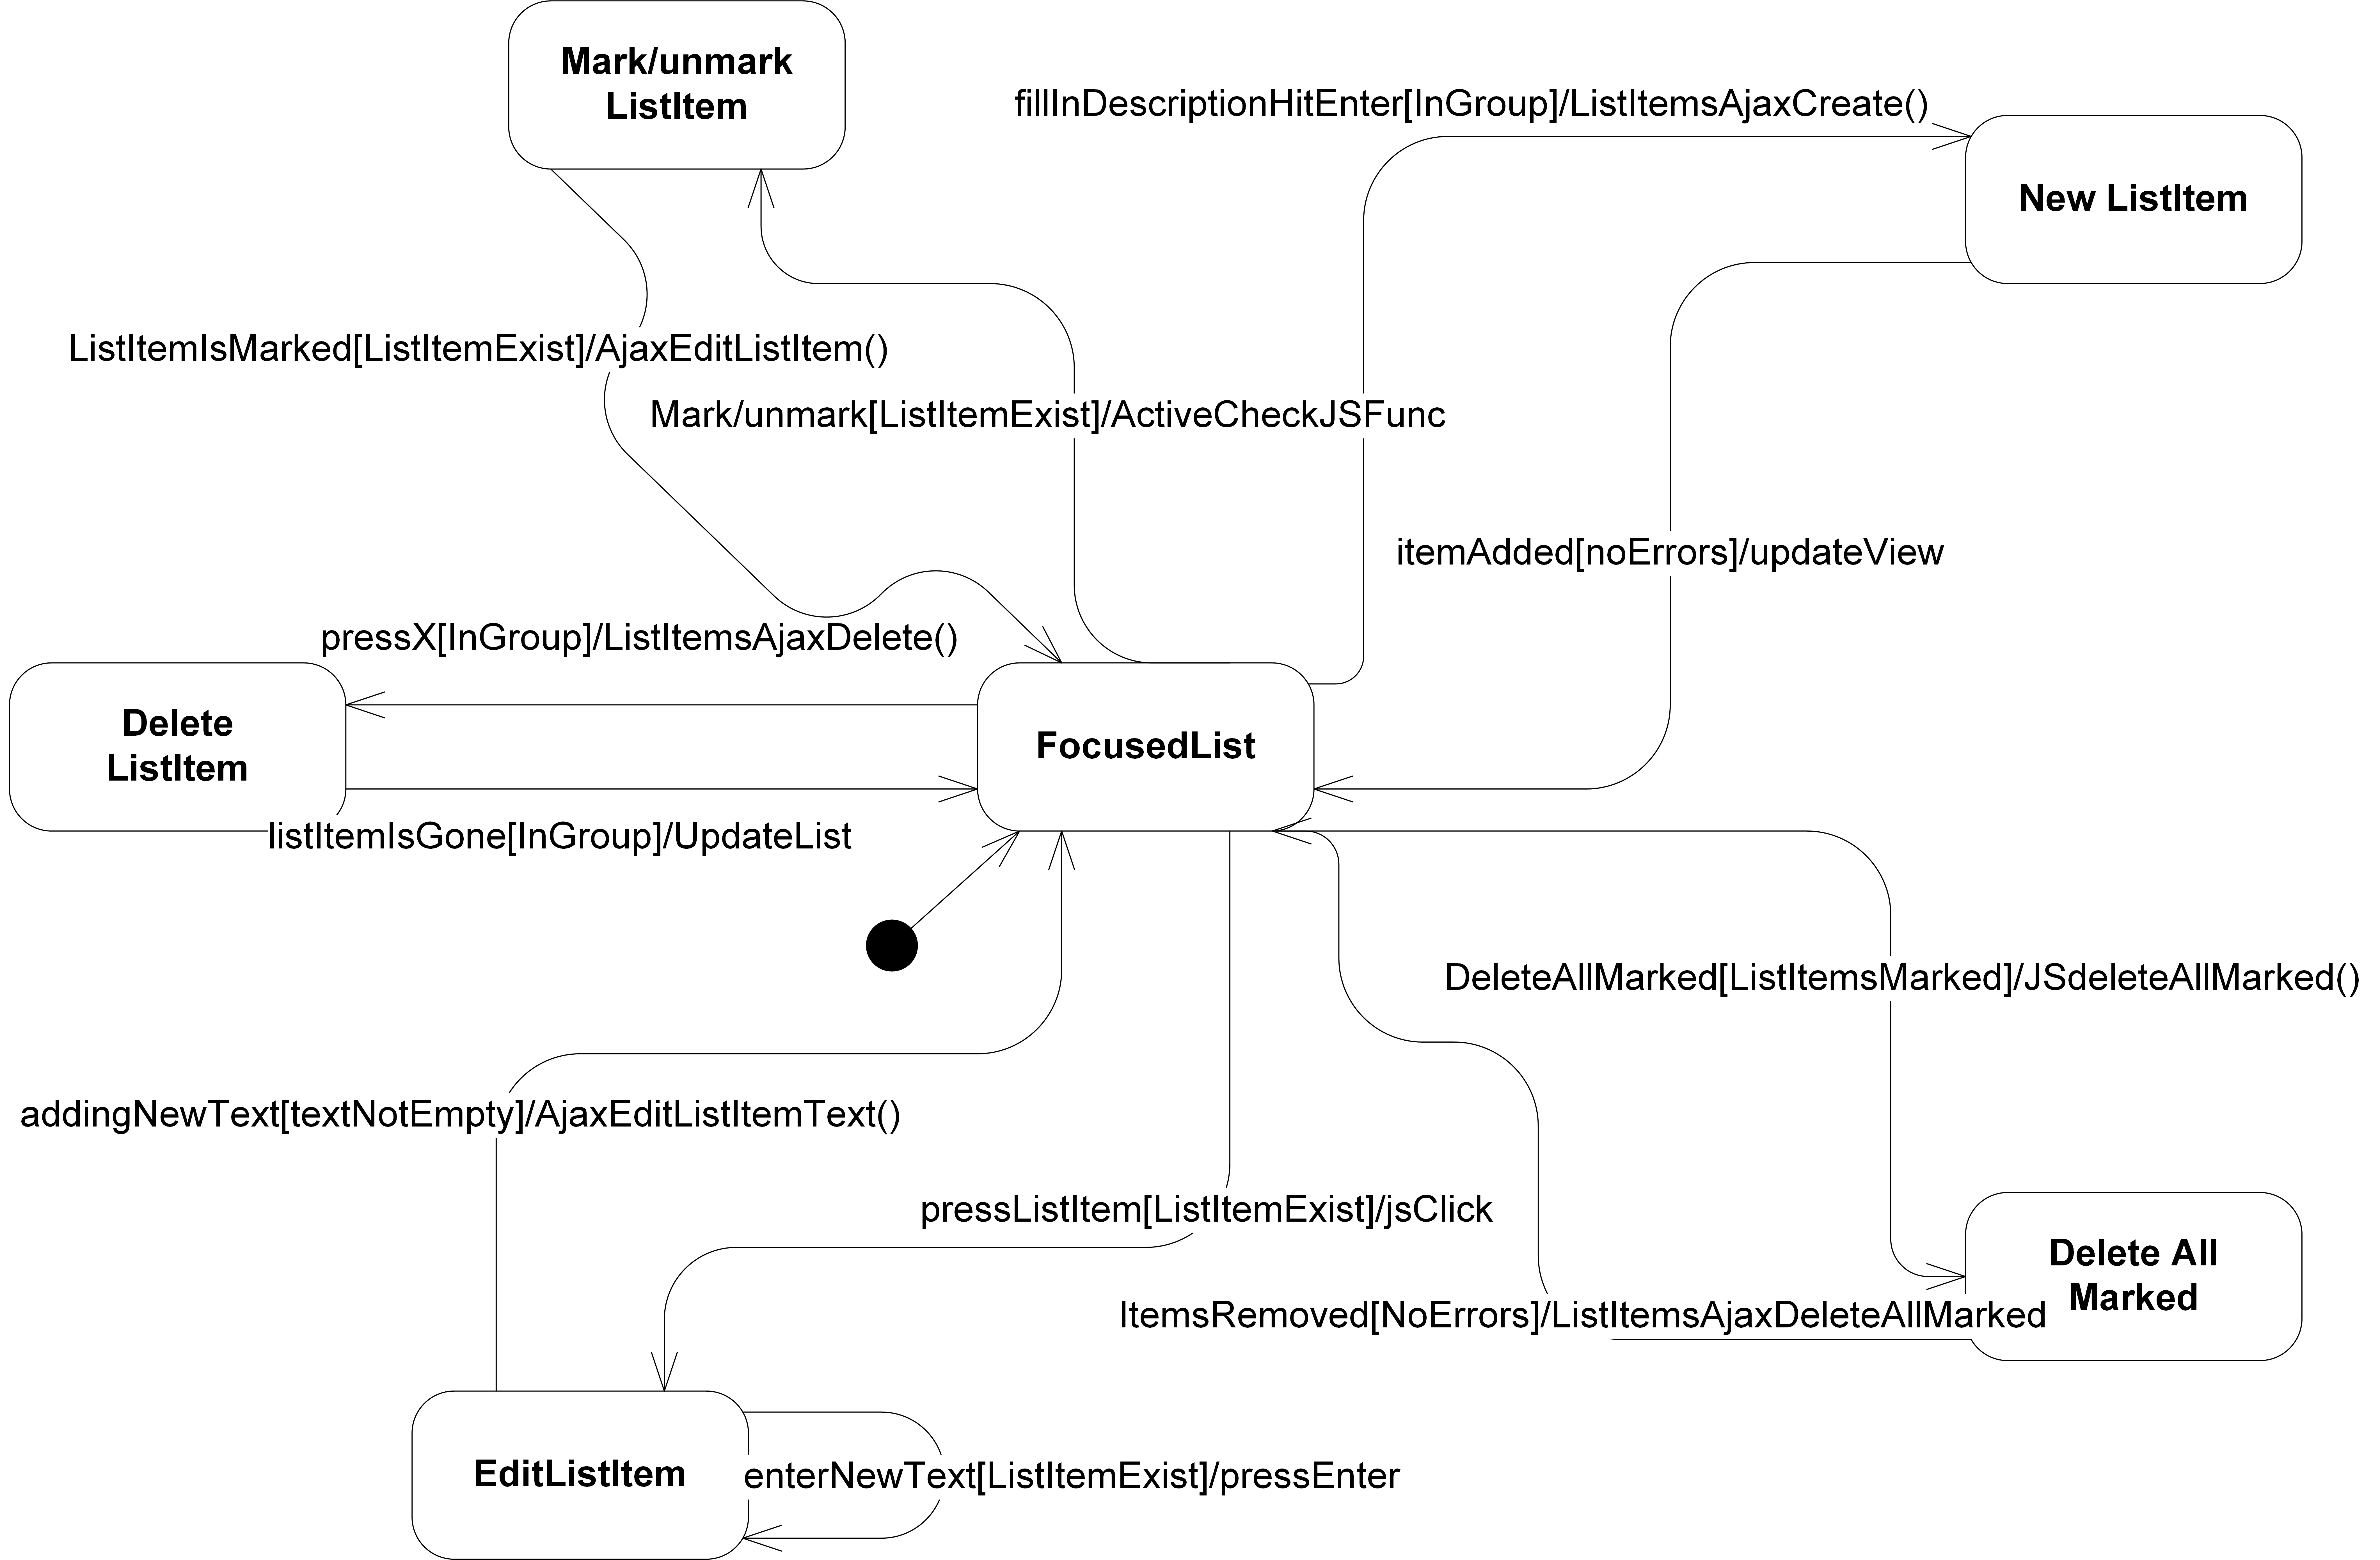
\includegraphics[width=\linewidth]{09_Arkitektur/Lists/Images/List_SM.png}
    \caption{Denne state machine viser hvilke funktionaliteter der er mulige at gøre med en widget af typen List. Dog er det valgt kun at gøre det muligt for skaberen af listen, at bruge funktionen med Delete All Marked. Dette kan dog nemt laves om, men blev bedømt til at være være lidt risikofyldt ellers.}
    \label{fig:list_stm}
\end{figure}

I bilagende er der lavet sekvensdiagrammer der demonstrerer disse funktionaliteter, hvor nogle er udeladt, da sekvenserne bliver meget ensformige. I stedet for at Delete All Marked kun kan gøres af ejer, kunne det evt ændres til at alle kan gøre det, men at de bliver spurgt om de er sikre på deres valg.
\section{Planning}\label{sec:Planning_arkitektur}

Planningwidget skal benyttes til planlægning af lige hvad man som bruger, har brugt for at planlægge. Derfor er det også væsentlig, at en planning kan konfigureres til brugerens behov. En planningwidget er tilknyttet en gruppe, men samtidig er den ikke nødvendigvis til alle gruppens medlemmer. Derfor skal der være muligt at tilføje/fjerne brugere til/fra en planning. Ud over disse overvejelser, så er der nogle US, som skal kunne gennemføres. Arkitekturen vil tage grundlag i disse US. Detaljerede US kan findes i bilag \cite{KravspecUserStoriesPlanning}.

\subsection{Data view}

\noindent Ud fra US tilknyttet planning, er nogle entities bestemt: Planning, Shift, UsersInPlanning, UsersShift og UserSwapShiftNotify. Disse skal udgøre tabellerne i databasen for planning. Hertil skal passende relationer bestemmes, så ledes, at en planning kan indeholde flere shifts, samt flere UsersInPlanning. UsersShift skal indeholde composite keys, bestående af UsersInPlanning id'er og Shift Id'er. 
\\ \\ 
UserSwapShiftNotify skal indeholde notifikationer for bytning af vagter mellem to brugere, hvortil passende attributer er blevet tilknyttet. Ud fra disse overvejelser er et ER-digram udarbejdet, som kan ses nedenfor på figur \ref{fig:ark_planning_data_dbview}.

\begin{figure}[H]
  \includegraphics[width=\linewidth]{09_Arkitektur/Planning/pictures/DB_Planning.jpg}
  \caption{ER Diagram for plannings til Database strukturen. OneToMany relationer fra planning til både Shift og UsersInPlanning. OneToMany fra Shift til UsersShift, samt fra UsersInPlanning til UsersShift. Samme relation benyttet til UserSwapShiftNotify.}
  \label{fig:ark_planning_data_dbview}
\end{figure}

\noindent Ud fra ER-diagrammet, er det muligt at designe modeller til planning.
\subsection{Logical view}\label{ssec:planlaegning:logicalview}
Dette afsnit skal forklare applikationslogikken for plannings i webapplikationen.
\\ \\
Bussiness logikken vil blive lagt i en controller, for at overholde MVC strukturen. Dertil vil PlanningControlleren komme til at stå for at håndtere brugers anmodninger og render views med modeldata. Til udarbejdelsen af arkitekturen for PlanningControlleren er der lagt vægt på US's, hvor der er arbejdet agilt med dokumentationen samt implementeringen. Dertil er ikke alle US implementeret endnu, men vil blive i fremtidige iterationer. \\

\noindent Ud fra arkitekturen beskrevet i bilag \cite{ArkitekturPlanning}, så er et klassediagram udarbejdet, som der kan tages udgangspunkt i til design og implementeringen. Klassediagrmmet ses nedenfor på figur \ref{fig:ark_planning_logic_classdiagram}.

\begin{figure}[H]
  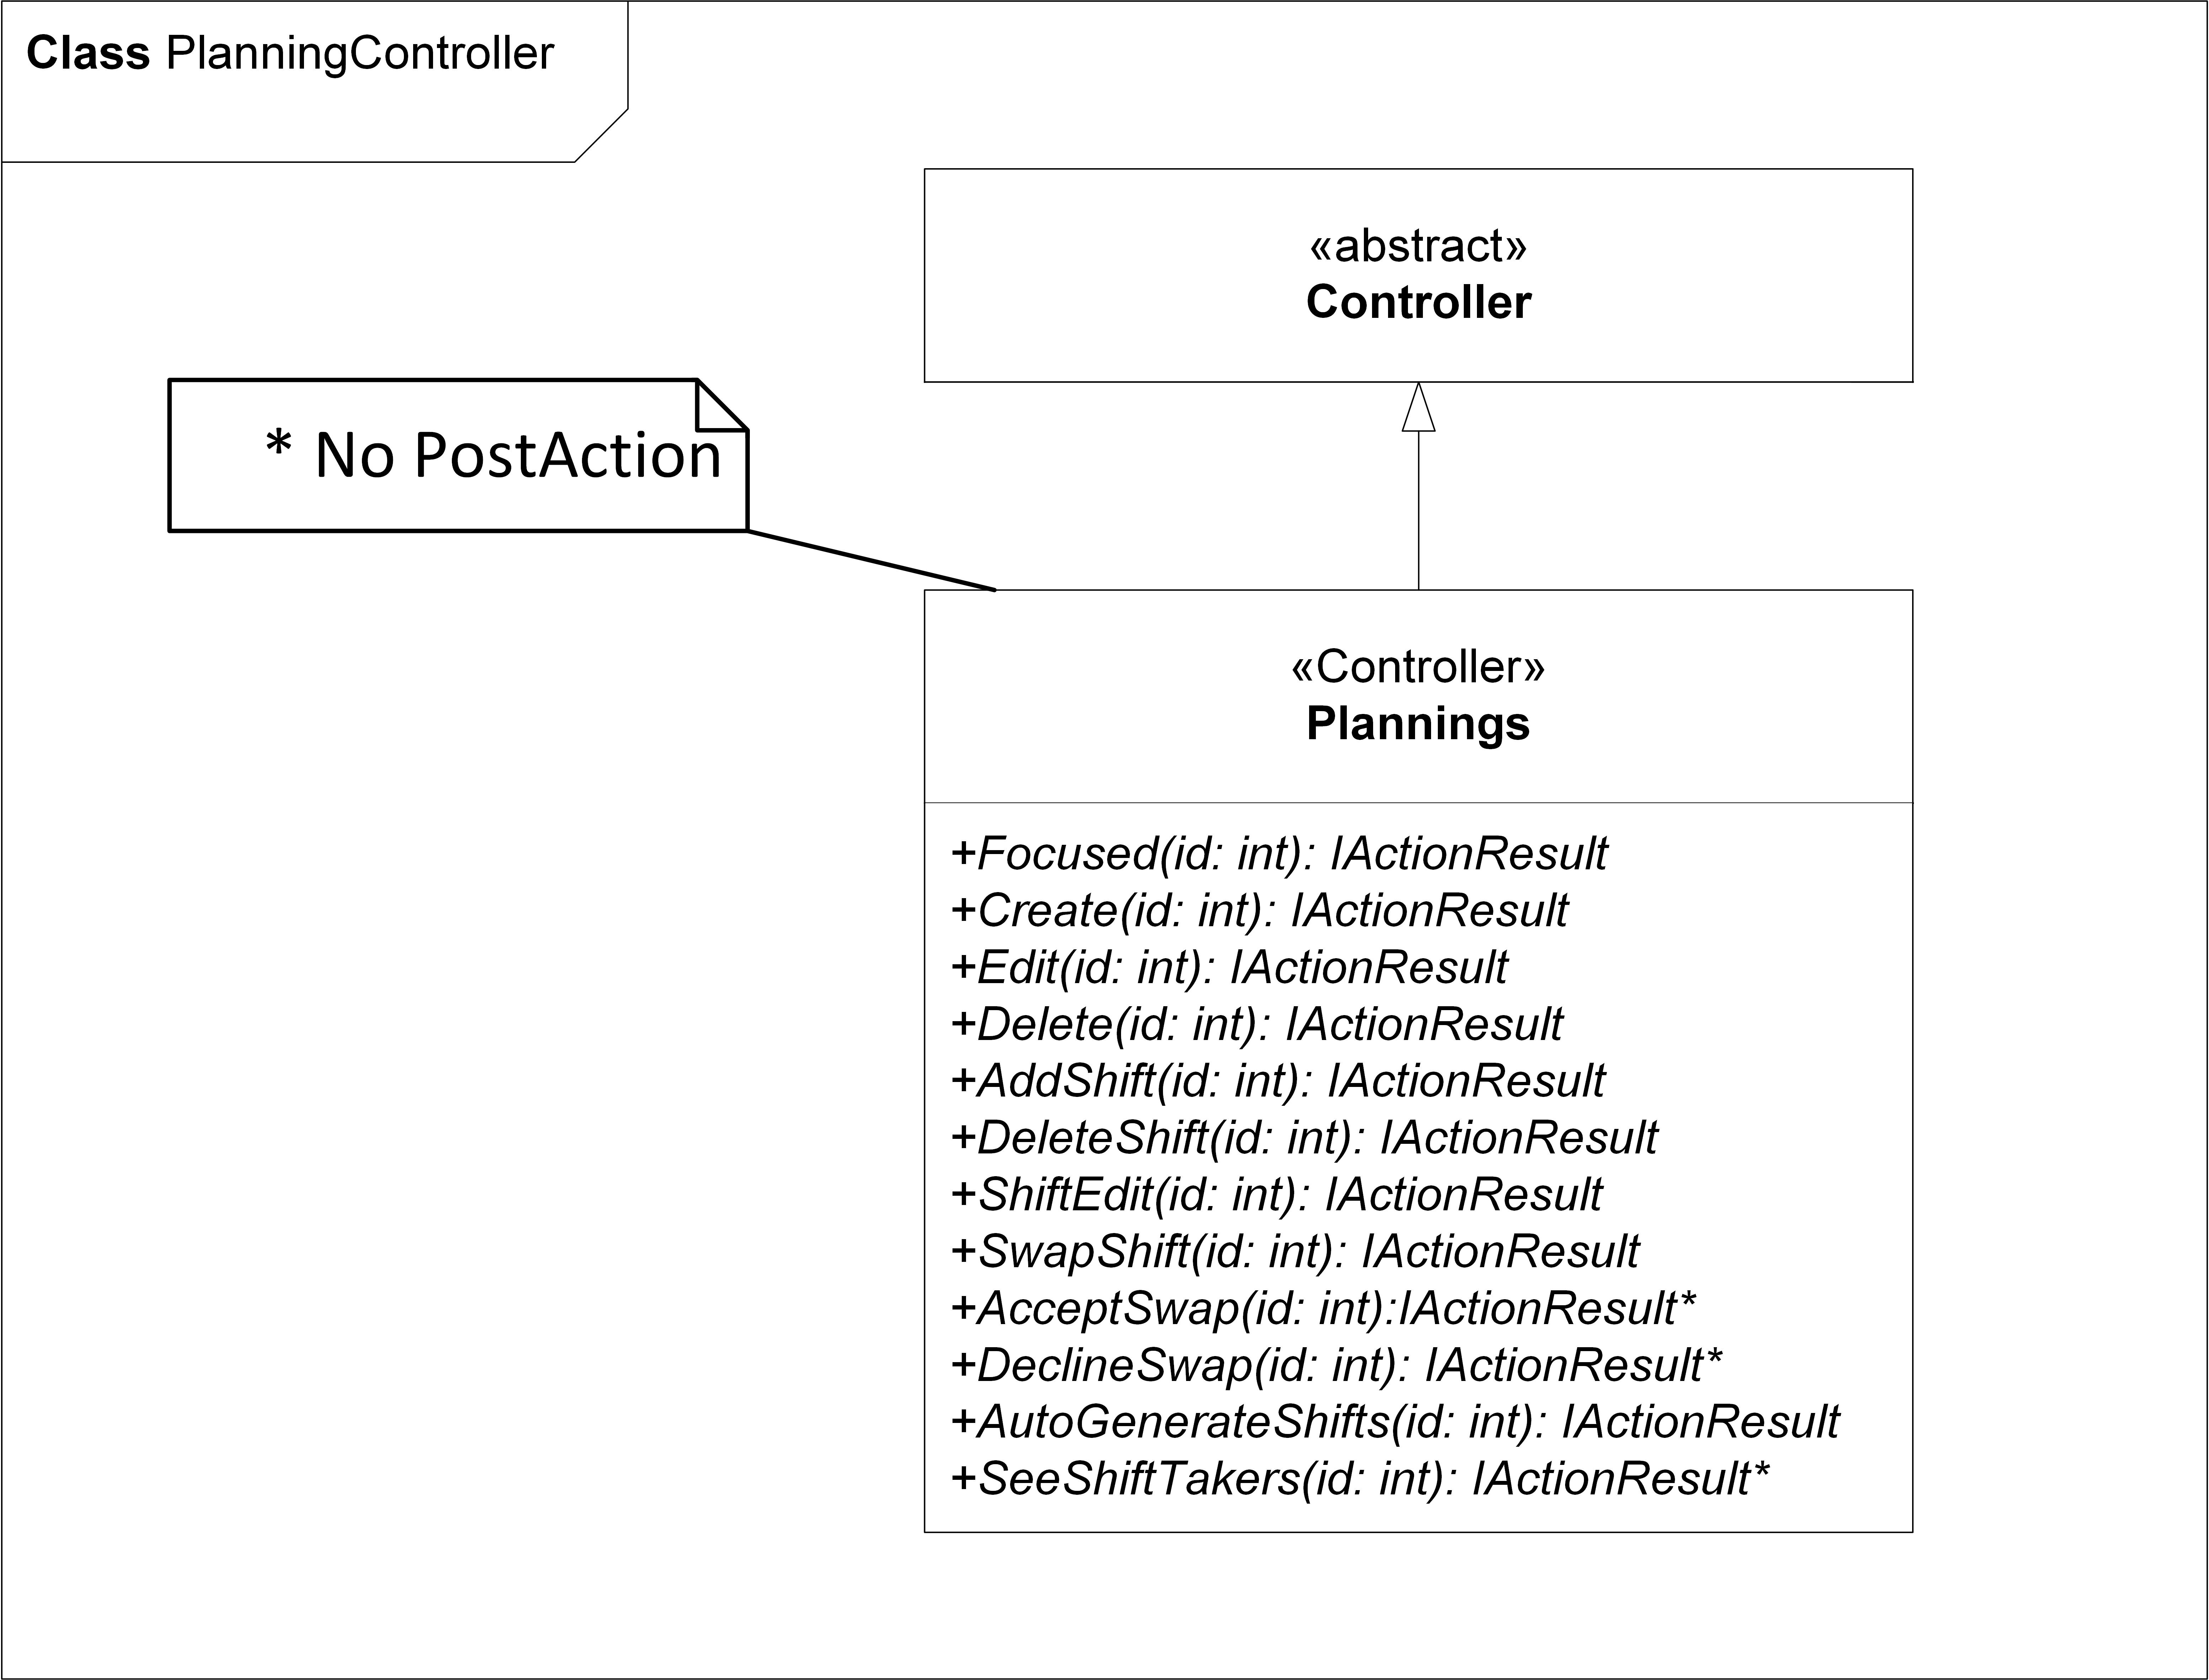
\includegraphics[scale=0.8]{09_Arkitektur/Planning/pictures/CD_Planning.jpg}
  \centering
  \caption{Klassediagram for planningController med de nødvendige metoder til at gennemføre de valgte US}
  \label{fig:ark_planning_logic_classdiagram}
\end{figure}



\section{Betaling}

I dette afsnit vil arkitekturen for widgettypen Betaling blive præsenteret. Dette vil ligge grundlag for at en uddybende beskrivelse af hvordan widget'en er designet og implementeret. 

\begin{figure}[H]
    \centering
    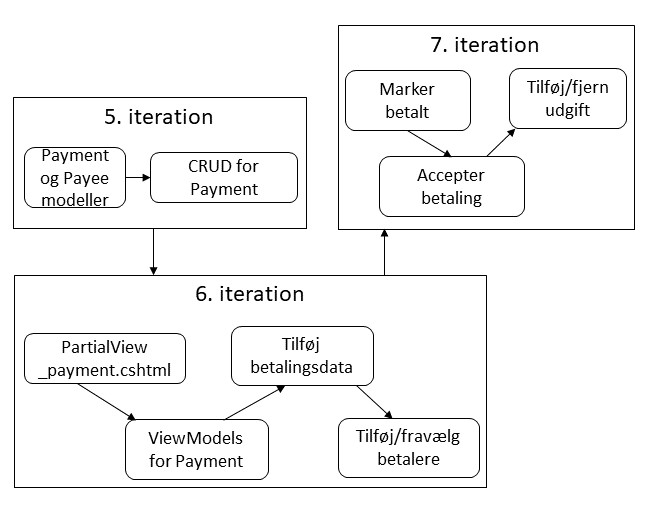
\includegraphics[width=\linewidth]{09_Arkitektur/Payment/Images/iteraionerCropped1.jpg}
    \caption{Der er blevet arbejdet på Betaling i de sidste uger i forløbet. Denne funktionalitet har kunnet blive implementeret direkte som en widget, og består også af en del JavaScript.}
    \label{fig:paymentIterations}
\end{figure}

\jonathan{Find ud af om det kan gøres lidt mindre når vi er ved at være færdige, så det kan være på en side}

Denne widget er vigtig for WePlanner på den måde at det i gruppe sammenhænge ofte er essentielt at kunne notere forskellige beløb der er blevet lagt ud for, og at kunne få et overblik over hvad andre har lagt ud for, så man kan få dem betalt.

\subsection{Data view}

En betaling består i WePlanners database af 2 modeller: Payment og Payees. For en Payment er der flere Payees, hvor Payees er Users, med ekstra attributter. De Users der skal være mulige at være Payees, skal være a typen GroupUsers, hvilket er en Model der er lavet i sammengængen med opsættelse af Groups. På baggrund af dette er dataen for Betalinger sat op på følgende måde.

\begin{figure}[H]
    \centering
    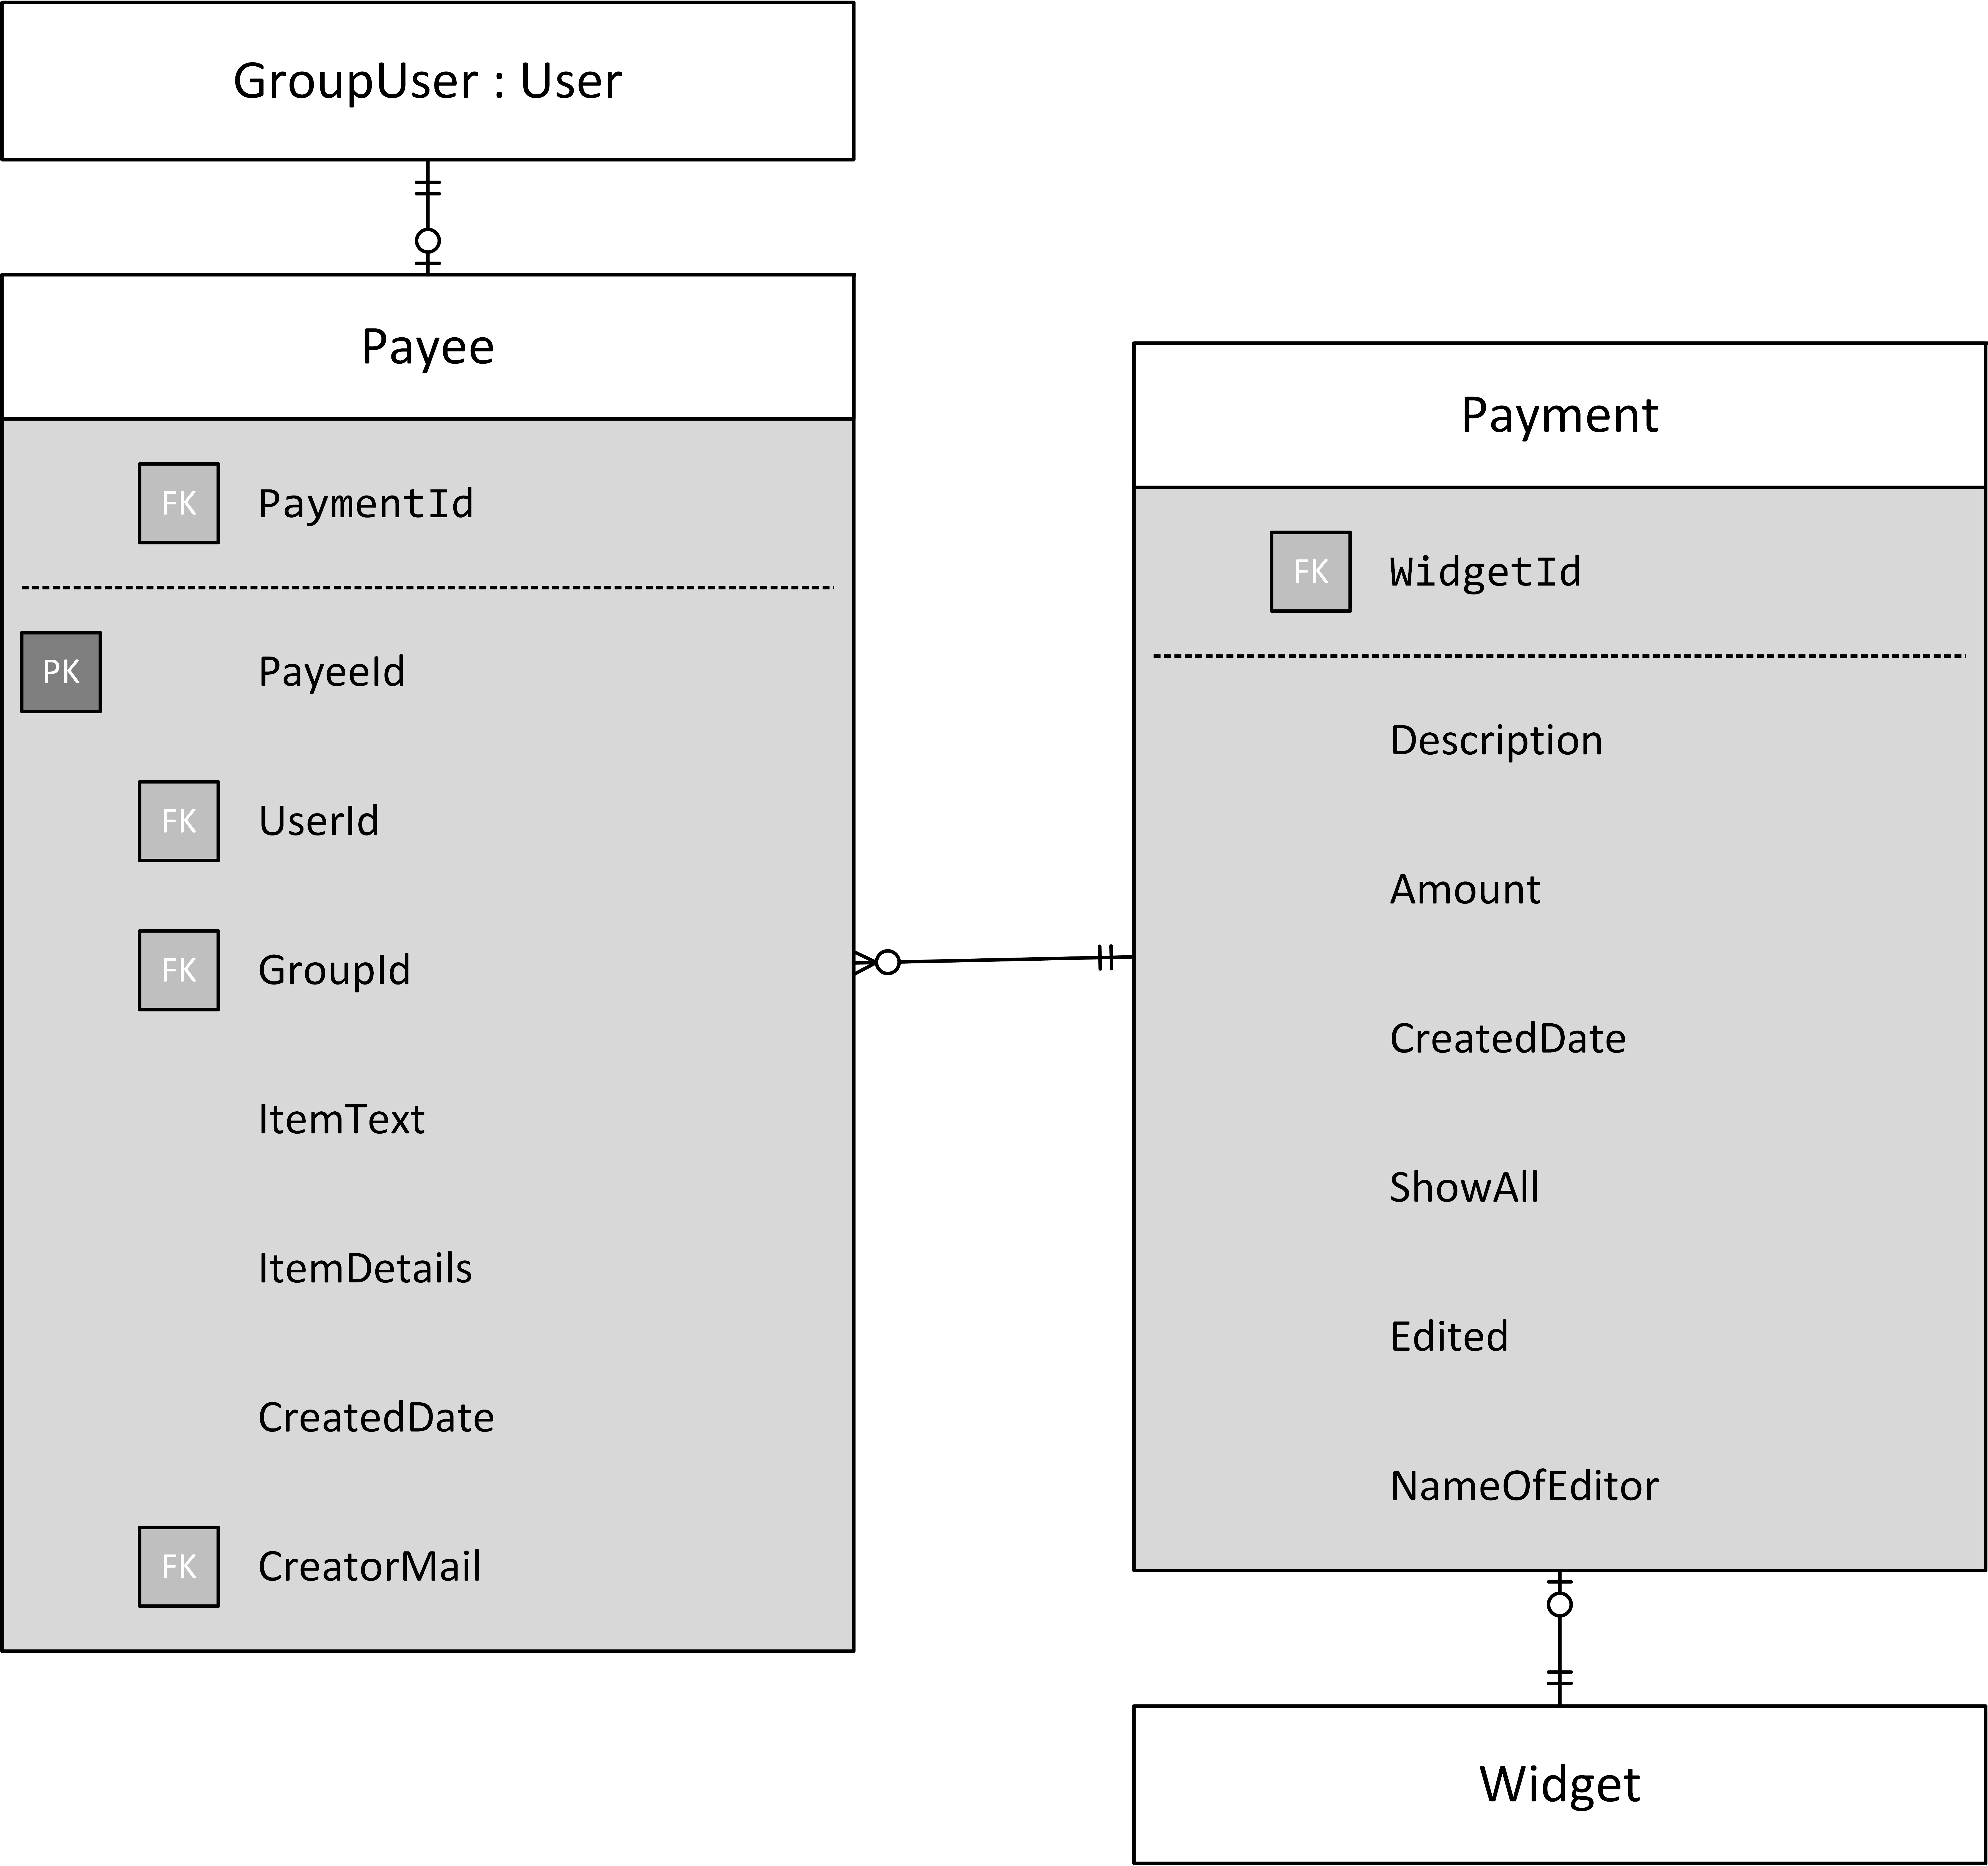
\includegraphics[width=\linewidth]{09_Arkitektur/Payment/Images/partialERDBetaling.png}
    \caption{Diagrammet viser dele af entitetsrelationerne mellem Payment og Payees, hvor det ses at Payment har en Widget, hvilket er vigtigt for WePlanners dashboard, som er gjort generelt for alle typer af Widgets.}
    \label{fig:betalingERD}
\end{figure}

For ovenstående Entity Relation diagram gælder det at en Payee har en GroupUser, hvor payee får alle denss vigtige brugerinformationer fra. Gennem GroupUser kan dder tilgås User, som der kan fås UserId, Email, Name etc. Disse bliver anvendt en del i Betaling, da det giver mere konfidentialitet at have information om brugeren, når der deles information om penge. Det fulde ER diagram kan ses i bilag om arkitektur for Betaling\cite{paymentPartERD}.

\subsection{Logical view}

Betalingen i WePlanner har lidt den samme funktionalitet som MobilePays underdel WeShare\cite{weShare}, som gør det muligt at dele udgifter med hindanden. Formålet med prototypen for WePlanner er på en måde at samle mange funktionaliteter et sted, hvor af en af funktionaliteterne er en slags WeShare. I fremtidige iterationer kunne det være en idé at undersøge muligheden for at kunne gå sammen med MobilePay of WeShare.\\

\noindent På nedenstående figur \ref{fig:paymentFunctionality}, ses hvad der kan gøres ud fra en Payment.

\begin{figure}[H]
    \centering
    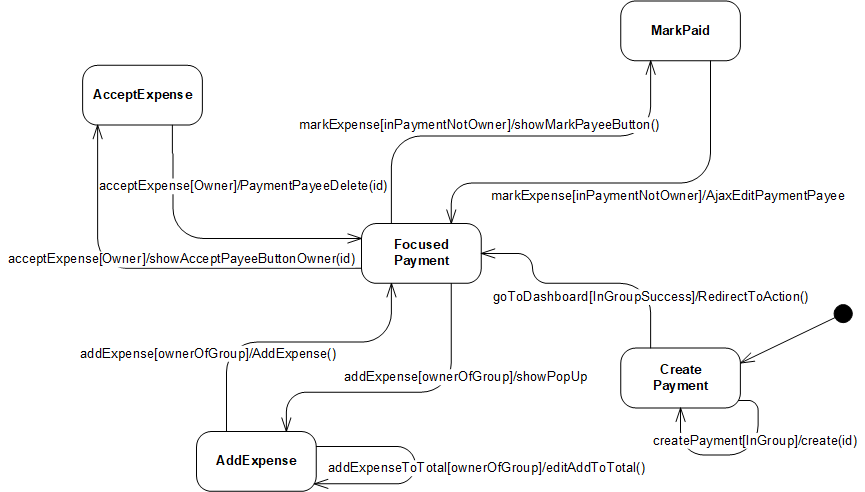
\includegraphics[width=\linewidth]{09_Arkitektur/Payment/Images/Payment_STM.png}
    \caption{Det ses at man ud fra en Payment kan Markerer som betalt, Accepter betaling og tilføj ny udgift. Hvordan dette gøres beskrives yderligere i design og implementering og mere detaljeret i projektets bilag.}
    \label{fig:paymentFunctionality}
\end{figure}

\jonathan{Ved ikke hvad jeg mere skal skrive... fml}
\section{Wall}
Wall-widgetten skal have mulighed for at oprette/slette/redigere en opslagstavle(Wall) og oprette/slette/redigere opslag (WallPost) til en specifik opslagstavle. Disse er essentielt set alle CRUD operationer. Desuden skal en opslagstavle kunne deles mellem flere grupper.

\subsection{Data view}
Indledningsvist oprettes to entitieter - Wall og WallPost, som bruges til at lave en tabel i databasen. Der er blevet besluttet at lave følgende struktur i databasen som kan ses på figur \ref{fig:Wall_ERDiagram}. På denne måde vil det blive muligt at tilføje WallPosts til en Wall, samt at oprette en Wall-widget.

\begin{figure}[H]
  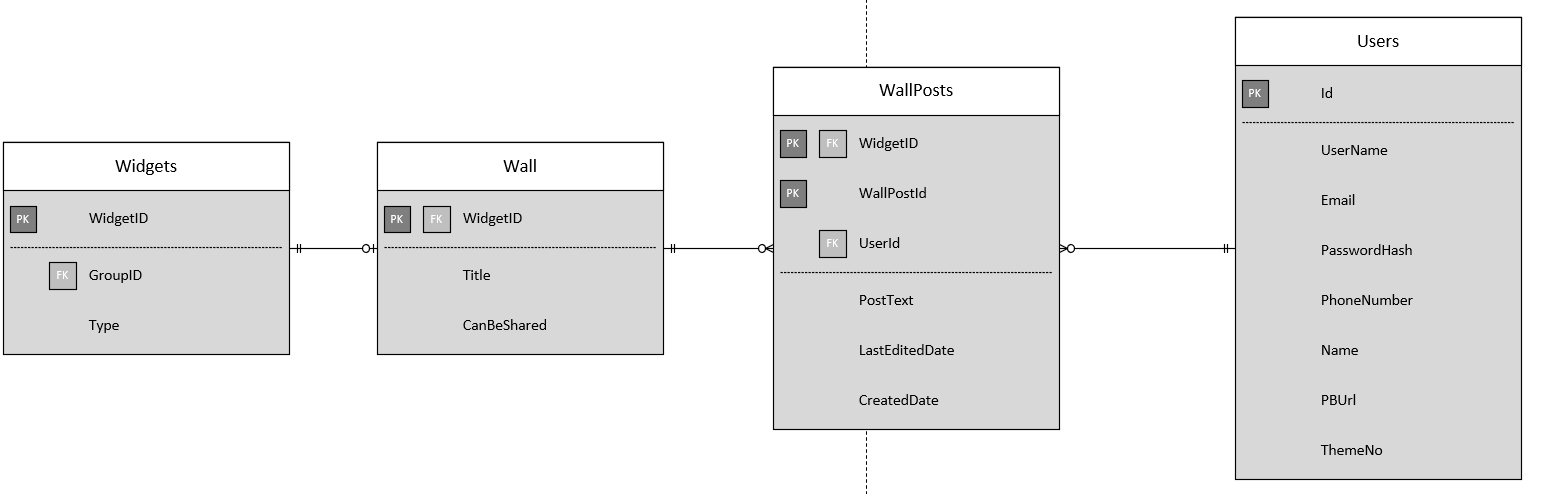
\includegraphics[width=1.0\linewidth]{01_Billeder/09_Arkitektur/Wall_DBArch.png}
  \caption{Færdige ER diagram over Wall. Denne strukture udvikles i 2. iteration, og forbliver den samme igennem udviklings processen. }
  \label{fig:Wall_ERDiagram}
\end{figure}

\jonathan{Du kunne godt trække Users lidt tættere på WallPosts så billedet kan blive lidt større?}

US'en der omhandler at kunne dele en opslagstavle med en anden grupper er der ikke lavet arkitetur for, da arbejdet på denne US ikke er påbegyndt endnu. Her ville det kræve at der blev oprettet en GroupsWalls tabel, der indeholder informationer om hvilke grupper der kan se hvilke Walls. 

\subsection{Logical view}
Logikken for denne del af systemet er forholdsvist simpel, og beskrives uddybende i bilag. Her er der dog lagt vægt på at brugere kun skal kunne tilgå de dele af Wall som de har tilgang til. Fx, skal det ikke være muligt for en hvilken som helst bruger at slette en anden brugers WallPost. I iteration 6, opdateres alt funktionalitet der opretter/sletter eller redigerer i enten WallPost eller Wall, til at vises i pop-up vinduer. Funktionaliteten i denne widget er forholdsvist lille, hvormed vurderes det at alt funktionaliteten kan tilgås fra widgetten på dashboard siden, uden at det bliver for uoverskueligt. Den færdige STM der bekriver de forskellige views og hvordan der kan laves om i dette, kan ses på figur \ref{fig:Wall_STM}.    

\begin{figure}[H]
  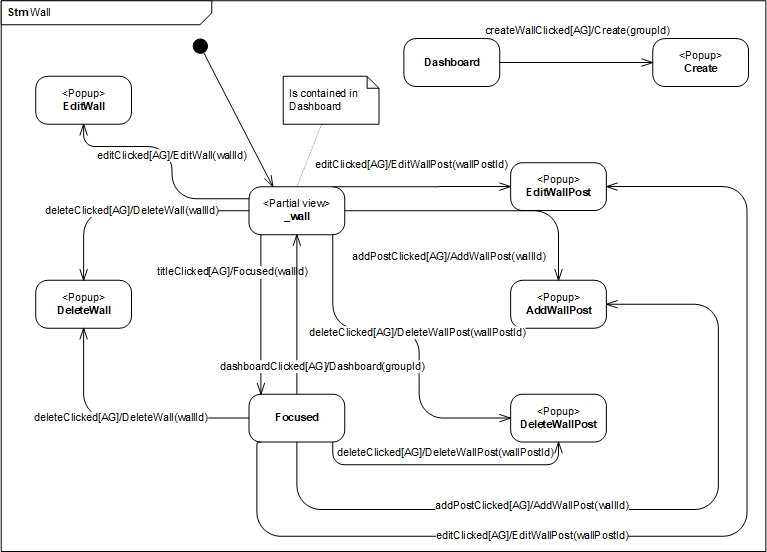
\includegraphics[width=1.0\linewidth]{01_Billeder/09_Arkitektur/Wall_STM.jpg}
  \caption{STM fra 6. iteration der viser hvordan der kan navigeres mellem forskellige views for at slette/redigere/oprette Wall, samt WallPosts. Når der trykkes på 'submit' knappen i et pop-up, laves der et postkald til en funktion af samme navn i WallControlleren. Herefter omdirigeres til det view som pilen peger på. Ordforklaring: AG - Access Granted}
  \label{fig:Wall_STM}
\end{figure}














\section{Deployment view}
I dette afsnit vil give et indblik til, hvordan softwaren er mappet til hardware, som i dette tilfælde vil være browsere, serveres og databaser. \\

\noindent Efter gennemgang af Data view og Logical view for alle dele af WePlanner, samles det hele i et Deployment view. Deployment view er det view, som viser, hvordan helheden af et projekt bliver implementeret i forhold til alle komponeneter. På nedenstående figur \ref{fig:ark_deploy_deploymentdiagram} ses det, hvilke komponenter WePlanner består af.

\begin{figure}[H]
  \includegraphics[width=\linewidth]{09_Arkitektur/Generelt_Deployment/deploymentDiagram.jpg}
  \centering
  \caption{Deployment diagram for hele systemet. Her er 3 dele, hvor client er browseren, som en bruger benyttet. Application serveren og DB server bliver hostet fra Unoeuro til domænet weplanner.}
  \label{fig:ark_deploy_deploymentdiagram}
\end{figure}

\noindent Som det kan ses på diagrammet, så er deployment delt op i 3 eksisterende stykker software, hvor koden kommer til at køre. Det første er client, som er browseren, hvori man tilgår webapplikationen. Browseren vil kommunikere med en web-/applikationsserver, hvor den egentlige sourcekode til planning er placeret. Denne server kommunikere sammen med browseren vha. en HTTP forbindelse. Webserveren indeholde så strukturen for mvc, plus wwwroot, som indeholder statisk kode, som f.eks. css og js filer, som views benytter. \\